\chapter{Livello applicazione}

La rete Internet, nelle sue componenti sia hardware che software, è stata progettata e sviluppata per fornire servizi a livello applicazione.\
Questi servizi vengono forniti agli utenti della rete dal quinto livello della pila di protocolli TCP/IP.\
Lo scopo degli altri livelli è rendere possibile questi servizi.

\section{Introduzione}

Il livello applicazione fornisce servizi all'utente.\
La comunicazione è fornita per mezzo di una connessione logica:\ questo significa che i livelli applicazione nei due lati della comunicazione agiscono come se esistesse un collegamento diretto (immaginario) attraverso il quale poter inviare e ricevere messaggi.

\subsection{Protocollo dello strato di applicazione}

Definisce
\begin{itemize}
    \item i \textbf{tipi di messaggi} scambiati a livello applicativo (es:\ di richiesta e di risposta)
    \item la \textbf{sintassi} dei vari tipi di messaggio (i campi del messaggio)
    \item la \textbf{semantica} dei campi (significato)
    \item le \textbf{regole} per determinare quando e come un processo invia messaggi o risponde ai messaggi
\end{itemize}

\subsection{Paradigmi del livello applicazione}

Dovrebbe ormai essere chiaro che per utilizzare Internet sono necessari due programmi che interagiscono l'uno con l'altro:\ uno eseguito su un certo computer in qualche parte del mondo, l'altro eseguito su un secondo computer in qualsiasi altro luogo.\
I due programmi hanno la necessità di scambiarsi i messaggi sfruttando l'infrastruttura di Internet.\
I due programmi applicativi devono essere entrambi in grado di richiedere e offrire servizi, oppure ciasuno deve occuparsi di uno dei due compiti? Con il passare del tempo, sono stati sviluppati due approcci (paradigmi) diversi:\ il paradigma client/server e quello peer-to-peer.

\subsubsection{\emph{Client/server:\ il paradigma tradizionale}}

L'approccio tradizionale è chiamato \emph{client/server}, ed è stato il paradigma più utilizzato fino a pochi anni fa.\
Con questo paradigma il fornitore di servizi è un programma applicativo chiamato processo \emph{server}, sempre in esecuzione in attesa che un altro programma applicativo, chiamato processo \emph{client}, apra una connessione via Internet e richieda un servizio.

\subsubsection{\emph{Peer-to-peer:\ il nuovo paradigma}}

Un nuovo approccio, chiamato \emph{paradigma peer-to-peer} (spesso abbreviato con paradigma P2P), è emerso come risposta alle necessità di alcune nuove applicazioni.\
In questo paradigma non è necessario che un processo server sia permanentemente in esecuzione in attesa che si connetta il processo client.\
Questa responsabilità viene condivisa tra i peer:\ un computer connesso a Internet può ricevere un servizio in un istante e offrire servizi in un altro momento.\
In alcuni casi, un computer può perfino fornire e ricevere servizi contemporaneamente.

\subsubsection{\emph{Paradigma misto}}

Un'applicazione può sfruttare un mix dei due paradigmi combinando i vantaggi di ciascuno di essi.

\section{Paradigma client/server}

Nel paradigma client/server la comunicazione a livello applicazione avviene tra due programmi applicativi in esecuzione chiamati \textbf{processi}:\ un \emph{client} e un \emph{server}.\
Un client è un programma in esecuzione che inizia la comunicazione inviando una richiesta; un server è altro programma applicativo che attende le richieste dai client.\
Il server gestisce le richieste ricevute dai client, prepara i risultati e li rispedisce da un client.\
Questa definizione implica che il server sia in esecuzione quando arriva una richiesta da un client, mentre il client può essere in esecuzione solamente quando necessario.

\subsection{API:\ Application Programming Interface}

Un programma è solitamente scritto in un linguaggio di programmazione con un insieme predefinito di istruzioni che indicano al computer le operazioni da eseguire.\
Se si vuole sviluppare un programma capace di comunicare con un altro programma, è necessario un nuovo insieme di istruzioni per chiedere ai primi quattro livelli dello stack TCP/IP di aprire la connessione, inviare/ricevere dati e chiudere la connessione.\
Un insieme di istruzioni di questo tipo viene chiamato \emph{API} (Application Programming Interface).\
Nella programmazione, un'interfaccia non è altro che un insieme di istruzioni usato per l'interazione tra due entità.\
In questo caso una delle entità è il processo a livello applicazione e l'altra è il sistema operativo che implementa i primi quattro livelli TCP/IP.\
Il produttore di un computer include i primi quattro livelli TCP/IP nel sistema operativo e fornisce le relative API.\
I processi eseguiti a livello applicazione sono così in grado di comunicare con il sistema operativo per inviare e ricevere messaggi via Internet.\
Sono state sviluppate diverse API di comunicazione, tra le quali l'\emph{interfaccia socket} (\emph{socket interface}).

\subsubsection{\emph{Socket}}

Sebbene una socket possa apparire come un terminale o un file, non è un'entità fisica di questo tipo:\ è un'astrazione.\
Si tratta in realtà di una \emph{struttura dati} creata e utilizzata dal programma applicativo.\
Si può dire che, per quanto riguarda il livello applicazione, comunicare fra un processo client e un processo server significa comunicare tra due socket create nei due lati della comunicazione.

Il client considera la socket come l'entità che riceve le richieste e fornisce le risposte; il server vede la socket come entità che gli sottopone le richieste e alla quale inviare le risposte.

\subsubsection{\emph{Socket address}}

L'interazione fra client e server è una comunicazione bidirezionale.\
Nella comunicazione bidirezionale si rende necessaria un coppia di indirizzi:\ \emph{locale} (mittente) e \emph{remoto} (destinatario).\
L'indirizzo locale in una direzione è l'indirizzo remoto nell'altra direzione e viceversa.\
Poiché la comunicazione nel paradigma client/server avviene fra due socket, è necessaria una coppia di socket address (indirizzo delle socket) per la comunicazione:\ un socket address locale ed uno remoto.

Un socket address deve innanzitutto identificare l'host sul quale il processo client o server è in esecuzione:\ un host in Internet viene definito univocamente dal proprio indirizzo IP, che solitamente è un intero a 32 bit.\
Ma sullo stesso computer potrebbero essere eseguiti contemporaneamente diversi processi client o server, di conseguenza è necessario utilizzare un altro identificatore per specificare il particolare client o server coinvolto nella comunicazione:\ un programma applicativo può essere identificato da un numero di porta, un intero a 16 bit.\
Un socket address sarà quindi composto dalla combinazione di un indirizzo IP e un numero di porta.

\subsection{Utilizzo dei servizi di livello trasporto}

Una coppia di processi fornisce servizi agli utenti di Internet, siano questi persone o applicazioni.\
La coppia dei processi, tuttavia, deve utilizzare i servizi offerti dal livello trasporto per la comunicazione, poiché non vi è una comunicazione fisica a livello applicazione.\
Nel livello trasporto dalla pila di protocolli TCP/IP sono previsti due protocolli principali:\ UDP e TCP.

\subsubsection{\emph{Protocollo UDP}}

UDP fornisce un servizio di trasferimento di datagrammi utente (user datagram) inaffidabile, privo di connessione (connectionless).\
L'assenza di connessione significa che non viene stabilita un'associazione logica fra i due lati della comunicazione che si scambiano i messaggi.\
Ogni messaggio è un'entità indipendente incapsulata in un pacchetto chiamato datagramma utente.\
Per UDP non esiste alcuna relazione (connessione) fra datagrammi utente consecutivi provenienti dalla medesima sorgente e diretti allo stesso destinatario.

UDP non è un protocollo affidabile.\
Sebbene possa cercare di verificare che i dati non vengano corrotti durante la trasmissione, non chiede al mittente di rispedire gli eventuali datagrammi utente corrotti o persi.\
Nonostante le limitazioni, UDP presenta dei vantaggi per alcune applicazioni, tra cui il fatto che sia un protocollo ``orientato al messaggio'', ovvero indichi in modo molto chiaro i confini dei messaggi trasmessi invece di creare un un unico flusso di comunicazione.

\subsubsection{\emph{Protocollo TCP}}

Il protocollo TCP fornisce un servizio basato su un flusso di byte (\emph{byte-stream}) affidabile e \emph{orientato alla connessione} (connection oriented).\
Prevede che le due entità in comunicazione stabiliscano per prima cosa una connessione logica scambiandosi alcuni pacchetti specifici per l'apertura della connessione.\
In questa fase, chiamata \emph{handshaking} (stretta di mano), le due entità stabiliscono alcuni parametri fra cui la dimensione dei pacchetti dati che potranno essere scambiati, la dimensione dei buffer necessari per memorizzare temporaneamente i dati durante la comunicazione e via così.\
Completata la fase di handshaking, le due entità possono inviarsi dati suddivisi in cosiddetti \emph{segmenti}, nelle due direzioni.\
Numerando i byte che vengono trasmessi, è possibile verificare la corretta sequenza dei byte ricevuti.\
Se per esempio alcuni byte risultassero persi o corrotti, il destinatario può richiederne la trasmissione, cosa che rende affidabile il protocollo TCP.

TCP è in grado di gestire anche il controllo del flusso e il controllo della congestione.\
Un inconveniente del protocollo TCP è il fatto di non essere orientato al messaggio, ovvero di non delimitare i messaggi scambiati bensì di fornire un flusso continuo di byte.\
È quindi un compito dell'applicazione quello di delimitare ed individuare i messaggi all'interno di questo flusso.

\subsubsection{Che tipo di trasporto è richiesto da un'applicazione?}

\begin{itemize}
    \item \textbf{Throughput}:\ tasso al quale il processo mittente può inviare bit al processo ricevente.
          \begin{itemize}
              \item alcune applicazioni (es.\ multimedia) richiedono un certo throughput minimo per essere efficaci
              \item altre apps (\emph{elastic apps}) possono far uso di poco o tanto throughput (a seconda di quanto ne trovano a disposizione)
          \end{itemize}
    \item \textbf{Perdita dei dati}
          \begin{itemize}
              \item alcune applicazioni (es.\ audio) possono tollerare alcune perdite
              \item altre applicazioni richiedono un trasferimento dati affidabile al 100\%
          \end{itemize}
    \item \textbf{Sensibilità ai ritardi}:\ alcune applicazioni (es.\ teleconferenza, giochi interattivi) richiedono un basso ritardo per essere efficaci
\end{itemize}

\section{Applicazioni client/server standard}

\subsection{World Wide Web e HTTP}

\subsubsection{\emph{World Wide Web}}

L'idea alla base del Web venne proposta per la prima volta da Tim Berners-Lee nel 1989 al CERN (Conseil Européen pour la Recherche Nucléaire) per consentire ai vari ricercatori sparsi nel mondo di accedere in modo facile alle pubblicazioni scientifiche.\
Il Web venne aperto al mondo commerciale nei primi anni '90.

Oggi il Web è un'enorme collezione di informazioni nella quale i documenti, chiamati \emph{pagine Web}, sono distribuiti in tutto il mondo e collegati l'uno all'altro come in una ragnatela.\
L'enorme diffusione e la crescita esplosiva del Web sono in stretta relazione con due termini nella frase precedente:\ \emph{distribuiti} e \emph{collegati}.\
La distribuzione favorisce la crescita del Web:\ qualsiasi server Web nel mondo può aggiungere un nuova pagina alla collezione e renderla disponibile a tutti gli utenti di Internet senza dover sovraccaricare un ipotetico server centralizzato.

Il collegamento delle pagine web è ottenuto tramite una tecnica chiamata \emph{hypertext} (ipertesto), che venne introdotta molti anni prima dell'avvento di Internet.\
Il concetto alla base dell'ipertesto è il collegamento (detto link).\
L'idea è quella di utilizzare una macchina in grado di recuperare automaticamente un documento memorizzato nel sistema ogni volta che viene incontrato un link al documento.\
Oggi l'espressione \emph{hypertext}, coniata proprio per indicare un insieme di documenti testuali collegati, è stata cambiata in \emph{hypermedia}, per indicare che una pagina può contenere documenti testuali così come immagini, clip audio e video.

\subsubsection{Uniform Resource Identifier}

Una URI è una forma generale (definita dagli standard IETF) per identificare una risorsa presente sulla rete.
\begin{itemize}
    \item \textbf{Uniform}:\ uniformità della sintassi dell'identificatore anche se i meccanismi per accedere alle risorse possono variare
    \item \textbf{Resource}:\ qualsiasi cosa abbia un'identità (documento, servizio, immagine, collezione di altre risorse)
    \item \textbf{Identifier}:\ informazioni che permettono di distinguere un oggetto da altri oggetti (entro un ambito definito di identificazione)
\end{itemize}
Ci sono due tipi di URI:
\begin{itemize}
    \item \textbf{Uniform Resource Locator (URL)}:\ sottoinsieme di URI che identifica le risorse attraverso il loro meccanismo di accesso (es.\ protocollo HTTP)
    \item \textbf{Uniform Resource Name (URN)}:\ sottoinsieme di URI che devono rimanere globalmente unici e persistente anche quando la risorsa cessa di esistere e diventa non disponibile
\end{itemize}

\subsubsection{\emph{URL (Uniform Resource Locator)}}

Una pagina Web, essendo un file, deve avere un identificatore univoco per distinguerla dalle altre pagine.\
Per identificare una pagina Web sono necessari tre identificatori:\ host, porta e percorso.\
Tuttavia, prima di definire la pagina Web è necessario indicare al browser quale applicazione client/server si desidera utilizzare, specificando il cosiddetto protocollo.\
Per identificare una pagina Web sono quindi necessari quattro parametri:\ il primo indica lo strumento che deve essere utilizzato per recuperare la pagina Web, la combinazione degli altri tre identifica l'oggetto ricercato (pagina Web).
\begin{itemize}
    \item \textbf{Protocollo}.\ Il primo identificatore è un'abbreviazione che indica il protocollo client/server necessario per il trasferimento.
    \item \textbf{Host}.\ L'identificatore dell'host può essere un indirizzo IP (in notazione decimale puntata) o il nome univoco assegnato al dominio di un host.
    \item \textbf{Porta}.\ La porta, un intero di 16 bit, è predefinito per molte applicazioni client/server standard.
    \item \textbf{Percorso}.\ Il percorso identifica la posizione e il nome del file nel filesystem.\ Il formato di questo identificatore dipende normalmente dal sistema operativo utilizzato.
\end{itemize}
Questi quattro elementi sono raggruppati assieme sotto la forma di \emph{URL}, come ad esempio:
\begin{itemize}
    \item \textbf{protocol://host/path} utilizzato nella maggior parte dei casi
    \item \textbf{protocol://host:porta/path} utlizzato quando è necessario specificare il numero di porta
\end{itemize}

\subsubsection{URI assoulute e relative}

Le URI possono essere assolute o relative
\begin{itemize}
    \item \textbf{URI assoluta}:\ identifica una risorsa indipendentemente dal contesto in cui è usata;
    \item \textbf{URI relativa}:\ informazioni per identificare una risorsa in relazione ad un'altra URL (è priva dello schema e della authority).
\end{itemize}
Le URI relative non viaggiano sulla rete, ma sono interpretate dal browser in relazione al documento di partenza.

\subsubsection{\emph{HTTP (HyperText Transfer Protocol)}}

HTTP (HyperText Transfer Protocol) è un protocollo che definisce come devono essere scritti i programmi client/server per accedere alle pagine Web.\
Un client HTTP invia una richiesta, un server HTTP restituisce una risposta.\
Il server utilizza la porta 80, il client utilizza un numero di porta effimero.\
HTTP sfrutta i servizi del TCP il quale, come visto in precedenza, è un protocollo affidabile e orientato alla connessione.\
Questo significa che, prima che possa avvenire una qualsiasi transazione, il client e il server devono stabilire una connessione.\
Al termine della transazione la connessione dovrebbe essere chiusa.\
Il client e il server non devono preoccuparsi degli eventuali errori nei messaggi scambiati o della perdita di dati, perché è il protocollo TCP che essendo affidabile si occupa di tutti questi aspetti.

HTTP è nato con un scopo generico, non solo quello di gestire l'ipertesto, ma volendo anche gestire sistemi basati sul concetto di oggetti o risorse distribuite.\
Ha un insieme di metodi di richiesta pensati espressamente per la condivisione e la collaborazione sugli ipertesti e tali metodi sono estendibili.\
È un protocollo \emph{stateless} (senza memoria di stato):\ le coppie richiesta/risposte sono indipendenti, cioè ogni richiesta viene eseguita indipendentemente da quelle che l'hanno preceduta.\
Inoltre, permette la rappresentazione e la negoziazione dei formati dei dati.

\subsubsection{Connessioni persistenti e non persistenti}

\textbf{Connessione}:\ un circuito logico di livello trasporto stabilito tra due programmi applicativi per comunicare tra loro.

La natura di ipertesto delle pagine Web può richiedere una serie di richieste e risposte.\
Se le pagine Web, gli oggetti ai quali si intende accedere, sono localizzate su server differenti, non vi è altra soluzione che creare una connessione TCP per ogni server e ottenere ciascun oggetto richiesto.\
Tuttavia, se più oggetti sono localizzati sullo stesso server, esistono due possibilità:\ recuperare ciascun oggetto usando una nuova connessione TCP o recuperare tutti gli oggetti con un'unica connessione.\
Il primo metodo viene indicato con l'espressione \emph{connessioni non persistenti}, il secondo metodo con \emph{connessioni persistenti}.\
HTTP nelle versioni precedenti alla 1.1 utilizzava connessioni non persistenti.\
Questo è cambiato in HTTP 1.1 dove le connessioni sono solitamente persistenti, ma l'utente può decidere diversamente.
\begin{itemize}
    \item \textbf{\emph{Connessione non persistente}}:\ viene stabilita una nuova connessione TCP per ciascuna coppia richiesta/risposta.
    \item \textbf{\emph{Connessione persistente}}:\ in questo caso il server, dopo aver mandato una prima risposta, lascia la connessione aperta in attesa di ulteriori richieste.\
          Il server può chiudere la connessione su richiesta del client o allo scadere di un timeout.
\end{itemize}
L'impiego di connessioni persistenti consente di risparmiare tempo e risorse.\
Infatti il tempo necessario per l'apertura e la chiusura di un gran numero di connessioni viene eliminato.\
Inoltre si ha una gestione più efficace del controllo di congestione:\ più tempo per regolare la frequenza di invio del traffico in base alla congestione di rete percepita.

\subsubsection{Pipelining}

Serve per migliorare ulteriormente le prestazioni.\
Consiste nell'invio da parte del client di molteplici richieste senza aspettare la ricezione di ciascuna risposta.
\begin{itemize}
    \item Il server \textbf{deve} inviare le risposte nello stesso ordine in cui sono state ricevute le risposte.\
          Se una richiesta richiede tempo per essere processata, le risposte alle richieste successive sono bloccate (\emph{Head of line blocking})
    \item Il client non può inviare in pipeline richieste che usano metodi HTTP non \emph{idem-potenti}.
\end{itemize}
Server Web che rispettano HTTP 1.1 devono supportare il pipelining, tuttavia è implementato in pochi browser.

\subsubsection{\emph{Formato dei messaggi}}

Il protocollo HTTP definisce il formato dei messaggi di richiesta e di risposta.\
Ogni messaggio è formato da quattro parti.\
La prima parte nel messaggio di richiesta viene chiamata \emph{riga di richiesta}, mentre nel messaggio di risposta viene chiamata \emph{riga di stato}.\
Le altre tre parti hanno lo stesso nome in entrambi i tipi di messaggio, ma le similarità si limitano al nome, poiché possono avere contenuti diversi.

\subsubsection{\emph{Messaggio di richiesta}}

Nella riga di richiesta vi sono tre campi separati da uno spazio e terminati da due caratteri (ritorno carrello e fine linea).\
I campi sono
\begin{itemize}
    \item \textbf{metodo}:\ definisce i tipi di richiesta.
    \item \textbf{URL}:\ definisce l'indirizzo e il nome della pagina Web corrispondente.
    \item \textbf{versione}:\ indica la versione del protocollo
\end{itemize}
Dopodiché posso avere più \emph{linee di intestazione} nelle quali ho il nome del campo e un valore, separati da uno spazio, seguiti da ritorno carrello e fine linea.\
Infine, preceduto da una linea vuota, vi è il \emph{corpo dell'entità}

\subsubsection{Header}

Gli \emph{header} sono insiemi di coppie (nome:valore) che specificano alcuni parametri del messaggio trasmesso o ricevuto:
\begin{itemize}
    \item \textbf{\emph{General Header}}:\ relativi alla trasmissione; per esempio data, codifica, connessione, \dots
    \item \textbf{\emph{Entity Header}}:\ relativi all'entità trasmessa; per esempio content-type, content-length, data di scadenza, \dots
    \item \textbf{\emph{Request Header}}:\ relativi alla richiesta; per esempio chi fa la richiesta, a chi viene fatta, che tipo di caretteristiche il client è in grado di accettare, autorizzazione, \dots
    \item \textbf{\emph{Response Header}}:\ nel messaggio di risposta; per esempio server, autorizzazione richiesta, \dots
\end{itemize}

\subsubsection{\emph{Messaggio di risposta}}

La prima riga di un messaggio di risposta è chiamata riga di stato.\
In questa riga vi sono tre campi separati da spazi e terminati da ritorno carello e fine linea.\
Il primo campo indica la versione del protocollo HTTP.\
Il campo di stato (\emph{status code}) definisce lo stato della richiesta, ed è costituito da tre cifre.\
La frase di stato esplicita in forma testuale il significato del codice.

\subsubsection{Status code}

\begin{center}
    \begin{tabular}{|c|m{21em}|}
        \hline
        \textbf{1xx:\ Informational} & Request received, continuing process                           \\
        \hline
        \textbf{2xx:\ Success}       & The action was successfully received, understood, and accepted \\
        \hline
        \textbf{3xx:\ Redirection}   & Further action must be taken in order to complete the request  \\
        \hline
        \textbf{4xx:\ Client Error}  & The request contains bad syntax or cannot be fulfilled         \\
        \hline
        \textbf{5xx:\ Server Error}  & The server failed to fulfill an apparently valid request       \\
        \hline
    \end{tabular}
\end{center}

\subsubsection{Content negotiation}

Le risorse possono essere disponibili in più rappresentazioni (lingua, formato di dati, dimensione, etc.).

\textbf{\emph{Content negotiation}}:\ meccanismo per selezionare la rappresentazione appropriata quando viene servita una richiesta (uso di Request e Entity headers).

\subsubsection{Metodi di HTTP}

\begin{center}
    \begin{tabular}{|c|l|}
        \hline
        \emph{Metodo} & \emph{Azione}                                           \\
        \hline
        GET           & Richiede un documento al server                         \\
        \hline
        HEAD          & Richiede le informazioni relative a un documento        \\
        \hline
        PUT           & Invia un documento dal client al server                 \\
        \hline
        POST          & Invia informazioni dal client al server                 \\
        \hline
        TRACE         & Restituisce una copia della richiesta inviata           \\
        \hline
        DELETE        & Elimina la pagina Web                                   \\
        \hline
        OPTIONS       & Richiede informazioni relative alle opzioni disponibili \\
        \hline
    \end{tabular}
\end{center}

\subsubsection{Metodi sicuri e idem-potenti}

\begin{itemize}
    \item \textbf{Safe methods}:\ metodi che non hanno effetti ``collaterali'', es.\
          non modificano la risorsa
          \begin{itemize}
              \item GET, HEAD, OPTIONS, TRACE
          \end{itemize}
    \item \textbf{Idem-potent methods}:\ i metodi possono avere la proprietà di \emph{idem-potenza} negli effetti collaterali se $N>0$ richieste identiche hanno lo stesso effetto di una richiesta singola
          \begin{itemize}
              \item GET, HEAD, PUT, DELETE, OPTIONS, TRACE
          \end{itemize}
\end{itemize}

\subsubsection{\emph{Web caching:\ il server proxy}}

HTTP supporta i \emph{server proxy}, ovvero dei computer che conservano una copia delle risposte alle richieste recenti.\
Il client HTTP invia una richiesta al server proxy, il quale controlla nella propria memoria cache.\
Se la risposta non è già presente nella cache, il proxy invia la richiesta al server corrispondente.\
Quando, in seguito, il proxy riceve la risposta, oltre a inviarla al client che l'aveva richiesta la memorizza anche nella propria cache, per renderla disponibile ad altri client che dovessero effettuare la stessa richiesta.

Il server proxy riduce il carico sul server originale, spesso riduce il traffico in rete e la latenza.\
Naturalmente il client, per poter utilizzare il server proxy, deve essere configurato in modo da accedere al proxy anziché direttamente al server Web.

Si noti che il server proxy agisce sia da server sia da client.\
Quando riceve una richiesta da un client per il quale ha una risposta, agisce come server inviando la risposta al client.\
Quando riceve una richiesta da un client per il quale non ha risposta, agisce prima come client inviando la richiesta al server Web, successivamente, quando riceve la risposta, agisce come server e invia la risposta al client.

\subsubsection{\emph{Cookie}}

Il Web è stato inizialmente progettato come ambiente ``senza stato'' (stateless):\ il server risponde alle richieste inviate dal client senza mantenere alcuna traccia del contesto, senza memorizzare alcuna informazione relativa alla sequenza di richieste inviate dal client, che sono quindi totalmente isolate.\
Questa modalità è perfettamente in linea con gli obiettivi iniziali del Web:\ poter ottenere facilmente documenti pubblicamente disponibili.\
Questo approccio oggi è decisamente inadeguato, visto che il Web ha anche altre funzioni:
\begin{itemize}
    \item alcuni siti Web sono usati per il commercio elettronico in negozi virtuali;
    \item alcuni siti Web devono limitare l'accesso ai soli utenti registrati;
    \item altri siti Web sono utilizzati come portali;
    \item altri siti ancora sono utilizzati a scopo pubblicitario.
\end{itemize}

\subsubsection{Creazione e memorizzazione dei cookie}

I dettagli relativi alla creazione e alla memorizzazione dei cookie variano molto a seconda dell'implementazione, ma il meccanismo di massima è sempre lo stesso:
\begin{itemize}
    \item il server quando riceve una richiesta memorizza le informazioni (relative al client) in una stringa o in un file.\ Tali informazioni possono comprendere il nome di dominio del client, i contenuti di un cookie precedente inviato dal client insieme alla richiesta (informazioni precedentemente raccolte dal server sul client quali nome, numero di registrazione, e così via), l'orario e altro;
    \item il server include il cookie nella risposta che invia al client;
    \item il browser che riceve la risposta memorizza il cookie in una directory adibita a questo scopo, a sua volta suddivisa per nome di dominio del server.
\end{itemize}

\subsubsection{Utilizzo dei cookie}

Quando un client invia una richiesta a un server, controlla nella directory dei cookie l'eventuale presenza di un cookie precedentemente inviato dal server.\
Il cookie eventualmente trovato viene incluso nella richiesta; il server che la riceve in questo modo capisce che si tratta di un vecchio client, già visto in precedenza.\
Si noti che i contenuti del cookie non sono mai mal interpretati dal browser o resi disponibili all'utente:\ il cookie è ``preparato'' e ``consumato'' dal server.

\subsection{TELNET}

Un programma server può fornire un servizio specifico al corrispondente programma client.\
È tuttavia improponibile avere una coppia client/server per ogni tipo di servizio, il numero di server crescerebbe a dismisura.\
In altre parole si tratta di un approccio non scalabile.\
È decisamente più ragionevole creare una coppia di applicativi client/server che permetta a un utente di accedere su un computer remoto e quindi di utilizzare tutti gli applicativi già presenti sul server.

TELNET, abbreviazione di TErminal NETwork, è uno dei primi protocolli di login remoto.\
L'accesso al server richiede nome utente e password ma il protocollo è estremamente vulnerabile agli attacchi di sicurezza in quanto tutte le informazioni, comprese le credenziali di accesso sono trasmesse in chiaro (senza alcuna forma di crittografia).\
Questo significa che un attaccante potrebbe semplicemente intercettare le credenziali ed ottenere l'accesso al sistema remoto.\
Per questo motivo, attualmente si usa prevalentemente un altro protocollo chiamato Secure Shell (SSH).

\subsubsection{\emph{Login locale e remoto}}

L'azione con la quale un utente si collega a un computer locale è detta \emph{login locale}.\
Se l'utente preme un tasto della tastiera connessa a un terminale del sistema, il carattere viene inviato al driver del terminale che a sua volta lo trasmette al sistema operativo del calcolatore; il sistema operativo, infine, interpreta la sequenza di caratteri ricevuti e invoca il programma applicativo richiesto all'utente.

Tuttavia, gli utenti che vogliano utilizzare programmi applicativi su dispositivi remoti devono effettuare un \emph{login remoto}, per esempio per mezzo della coppia client/server TELNET.\
I caratteri introdotti dall'utente vengono accettati dal driver del terminale e inviati al client TELNET che trasfoma la sequenza in una successione di caratteri con una codifica standard, che viene poi trasmessa allo stack TCP/IP locale.

I comandi o i messaggi di testo che viaggiano attraverso Internet e giungono allo stack TCP/IP del dispositivo remoto, dove vengono trasmessi al sistema operativo e da questo al server TELNET.\
Quest'ultimo, infine, li trasforma in una sequenza di caratteri utilizzabile dalla macchina remota.\
A questo punto sorge una piccola complicazione data dal fatto che nel server non è presente un driver di terminale.\
I caratteri provenienti dal client non possono essere recapitati direttamente al sistema operativo remoto perché questo è in grado di accettare soltanto caratteri provenienti da un driver di un terminale, che è assente (nel sistema remoto non è presente alcun terminale).\
Per questa ragione viene aggiunto un ulteriore software, detto driver dello pseudoterminale, con il compito di accettare i caratteri dal server e di trasmetterli al sistema operativo.\
Dopo questo passaggio intermedio il sistema operativo consegna infine i caratteri all'applicazione opportuna.

\subsubsection{TELNET:\ NVT}

\textbf{Problema}:\ TELNET deve poter operare con il numero massimo di sistemi e quindi gestire dettagli di sistemi operativi eterogenei.\
I terminali possono differire gli uni dagli altri per:
\begin{itemize}
    \item il set e codifica di caratteri;
    \item la larghezza della linea e lunghezza della pagina;
    \item i tasti funzione individuati da diverse sequenze di caratteri (escape sequence), per esempio una diversa combinazione di tasti per interrompere un processo, caratteri ASCII diversi per terminare le righe di testo.
\end{itemize}
\textbf{Soluzione}:\ definizione di un terminale virtuale.\
Sulla rete si considera un unico terminale standard e in corrispondenza di ogni host, si effettuano la conversione da terminale locale a terminale virtuale e viceversa.

TELNET assume che sui due host sia in esecuzione un \textbf{\emph{Network Virtual Terminal} (NVT)}.\
La connessione TCP è instaurata tra questi due terminali NVT.

L'NVT è un dispositivo ``immaginario'' che fornisce una rappresentazione astratta di un terminale canonico.\
Gli host, sia client che server, traducono le loro caratteristiche locali così da apparire esternamente come un NVT e assumono che l'host remoto sia un NVT.

Il \emph{Network Virtual Terminal} definisce un set di caratteri e di comandi universale che permette di trasformare il set di caratteri in uso localmente in un set di caratteri universali.\
Lo standard prevede che i terminali NVT si scambino i dati in formato ASCII a 7-bit, però la comunicazione è a 8-bit:\ in questo modo si differenziano i dati dalle sequenze di comandi veri e propri.\
Inoltre, i comandi sono anticipati da un ottetto speciale con tutti i bit settati a 1 chiamato \emph{Interpret as Command} (IAC).\
Tale meccanismo si chiama \emph{inband signalling}:\ i comandi e i dati sono mandati sulla stessa connessione.

\subsection{Posta elettronica}

La posta elettronica (o e-mail) consente agli utenti di scambiarsi messaggi.\
La natura di questa applicazione è tuttavia differente da altre applicazioni trattate fino a questo momento.\
In un'applicazione come HTTP, il programma server è sempre in esecuzione, in attesa di una richiesta dal client.\
All'arrivo della richiesta, il server provvede a fornire il servizio richiesto.\
Vi sono una richiesta e un risposta.\
Nel caso della posta elettronica la situazione è differente:\ il destinatario di un messaggio potrebbe non essere disponibile ad accettare messaggi di posta in quel momento (utente impegnato o computer spento); quindi lo scambio del messaggio deve prevedere questo disaccoppiamento tra mittente e destinatario, un po' come succede nella posta tradizionale.

\subsubsection{\emph{Architettura}}

Per spiegare l'architettura della posta elettronica si prende come riferimento lo scenario illustrato nella Figura \ref{fig:Mail}.

\begin{figure}[H]
    \centering
    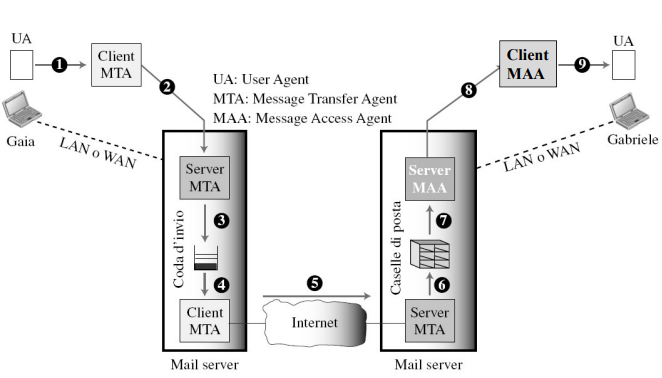
\includegraphics[width=\textwidth]{immagini/Mail_Elettronica.png}
    \caption{Scenario classico}
    \label{fig:Mail}
\end{figure}

Abitualmente il mittente e il destinatario della posta elettronica, Gaia e Gabriele, sono collegati via LAN o WAN a due server di posta.\
L'amministratore ha creato una \emph{mailbox} (casella di posta) per ogni utente dove memorizzare i messaggi ricevuti.\
Una mailbox non è altro che una porzione di spazio sulla memoria di massa del server, sottoforma di un file (o di una directory) con opportune restrizioni per far sì che solamente il proprietario possa accedere.\
Inoltre, l'amministratore ha creato anche una coda (spesso chiamata spool) dove memorizzare i messaggi in attesa di essere inviati.\
Gaia e Gabriele utilizzano tre \emph{agenti} differenti:\ un User Agent (UA), un Mail Transfer Agent (MTA) e un Message Access Agent (MAA).\
Gaia, per inviare un messaggio a Gabriele, utilizza un programma UA per preparare il messaggio e inviarlo al proprio server di posta.\
Quest'ultimo memorizza il messaggio in attesa di essere inviato all'interno di un'apposita coda.\
Il messaggio, tuttavia, deve essere inviato tramite Internet dal mail server di Gaia al mail server di Gabriele usando un MTA.\
Sono quindi necessari due MTA in ciascun mail server:\ uno client e uno server.\
Analogalmente alla maggior parte dei programmi client/server presenti in rete, il server deve essere in esecuzione permanente perché non può sapere quando il client richiederà una connessione.\
Il client, invece, può essere eseguito dal sistema quando in coda c'è un messaggio in attesa di essere spedito.\
L'user agent presso il sito di Gabriele gli consente di ricevere e leggere messaggi.\
Infine Gabriele utilizza un client MAA per ottenere i messaggi da un server MAA in esecuzione sul secondo server.

Ci sono due aspetti importanti da considerare.\
Primo Gabriele è obbligato a passare per il server di posta e non può utilizzare il server MTA direttamente.\
Per farlo, dovrebbe tenere il proprio computer costantemente acceso; nel caso in cui vi fosse connesso tramite WAN, dovrebbe mantenere la connessione attiva in permanenza:\ entrambe le situazioni sono improponibili.

Secondo, si noti che Gabriele richiede un'ulteriore coppia di programmi client-server:\ i programmi per accedere ai messaggi di posta.\
Il programma client-server MTA, infatti, è un'applicazione di tipo \emph{push}:\ il cliente ``spinge'' il messaggio al server.\
Gabriele invece richiede un programma di tipo \emph{pull}:\ il client deve ``tirare'' il messaggio dal server.

\subsubsection{Server postale (schema di principio)}

I mail server adottano una tecnica denominata \emph{spooling}:
\begin{itemize}
    \item L'utente invia un messaggio, il sistema ne pone una copia in memoria insieme all'id mittente, l'id destinatario, l'id della macchina di destinazione e il tempo di deposito.
    \item Il sistema avvia il trasferimento alla macchina remota.\
          Il sistema (cli\-ent) stabilisce una connessione TCP con la macchina destinazione.
    \item Se la connessione viene aperta, inizia il trasferimento del messaggio.
    \item Se il trasferimento va a buon fine il client cancella la copia locale della mail
    \item Se il trasferimento non va a buon fine, il processo di trasferimento scandisce periodicamente l'area di spooling, e tenta il trasferimento dei messaggi non consegnati.\
          Oltre un certo intervallo di tempo (definito dall'amministratore del server) se il messaggio non è stato consegnato, viene inviata una notifica all'utente mittente.
\end{itemize}

\subsubsection{\emph{Indirizzi}}

I sistemi che si occupano della consegna dei messaggi di posta elettronica necessitano di un sistema di indirizzamento che permetta di individuare in modo univoco gli utenti.\
In Internet, gli indirizzi di posta elettronica consistono in due parti:\ una parte locale e un nome di dominio (domain name), separati dal simbolo @.

La parte locale dell'indirizzo indica il nome di una mailbox in cui vengono memorizzati tutti i messaggi ricevuti dall'utente, in attesa che vengano prelevati dal client MAA.\
La seconda parte contiene il nome del dominio.\
Un'organizzazione sceglie uno o più host (a volte chiamati server di posta o mail exchanger) per la ricezione e l'invio della posta elettronica.

\subsubsection{\emph{User Agent}}

Il suo scopo è quello di semplificare all'utente il processo di invio e ricezione dei messaggi.\
Un user agent è un programma che consente di scrivere, leggere, rispondere e inoltrare i messaggi, ed è in grado inoltre di gestire le mailbox nei computer degli utenti.

\subsubsection{Message Transfer Agent:\ SMTP}

Si può affermare che la posta elettronica è una di quelle applicazioni che richiedono tre impieghi del paradigma client/server:\ la prima e la seconda sono MTA (Message Transfer Agent), la terza è un MAA (Message Access Agent).

Il protocollo che definisce in modo formale l'interazione tra il client e il server MTA è chiamato SMTP (\emph{Simple Mail Transfer Protocol}).\
SMTP è utilizzato in due diverse occasioni:\ fra mittente ed il suo server di posta e tra i due server di posta.\
L'obiettivo di SMTP è il \textbf{trasferimento affidabile e efficiente} di mail.\
È indipendente dal sistema di trasmissione usato e richiede solo il trasferimento di stream di byte ordinato e affidabile (l'RFC discute SMTP su TCP).

Una caratteristica di SMTP è la capacità di trasportare mail attraverso più reti.\
Un messaggio di mail può passare attraverso server intermedi nel percorso da mittente a destinatario finale.

Quando un client SMTP vuole trasferire un messaggio, stabilisce un \textbf{canale di trasmissione bidirezionale con un server SMTP}.\
La responsabilità di un client è di trasferire la mail a un server SMTP, o comunicare un eventuale insuccesso (\textbf{scambio formale di responsabilità}).\
Un client SMTP determina l'indirizzo di un host appropriato che ospita un server SMTP risolvendo il nome della destinazione in un mail server destinazione (risoluzione di un nome in indirizzo IP attraverso il DNS).

Possibili problemi che possono emergere nel trasferimento mail da un client a un server tramite SMTP:
\begin{itemize}
    \item connessione con mailserver del mittente (server inesistente o irraggiungibile)
    \item connessione con mailserver destinatario (server inesistente o irraggiungibile)
    \item inserimento in maibox destinatario (user unknown, mailbox full)
\end{itemize}
ma in tutti questi casi il mittente riceve una notifica.

Il destinatario può non ricevere il messaggio senza che il mittente sia avvisato solo se qualcuno (intruso, filtro antispam) rimuove il messaggio.

Quello che fa SMTP è semplicemente definire come deve avvenire l'interazione per mezzo di comandi e risposte:\ i comandi sono inviati da un client MTA a un server MTA, viceversa le risposte.\
I comandi terminano tutti con la medesima coppia di caratteri (ritorno carrello e fine linea).

\paragraph{Comandi} Il loro formato è composto da una keyword (parola chiave) e uno o più argomenti:

\begin{center}
    \textbf{Keyword}:\ argomento (o argomenti)
\end{center}

\begin{table}[H]
    \centering
    \begin{tabular}{|c|c|m{12em}|}
        \hline
        \emph{Keyword} & \emph{Argomenti}        & \emph{Descrizione}                                   \\
        \hline
        HELO           & Nome dell'host mittente & L'host mittente si identifica                        \\
        \hline
        MAIL FROM      & Mittente del messaggio  & Identifica il mittente del messaggio                 \\
        \hline
        RCPT TO        & Destinatario            & Identifica il destinatario del messaggio             \\
        \hline
        DATA           & Corpo del messaggio     & Invia il contenuto del messaggio                     \\
        \hline
        QUIT           &                         & Termina la sessione SMTP                             \\
        \hline
        RSET           &                         & Interrompe la transazione in atto                    \\
        \hline
        VRFY           & Nome del destinatario   & Verifica la validità dell'indirizzo del destinatario \\
        \hline
    \end{tabular}
\end{table}

\paragraph{Risposte} Costituite da un codice a tre cifre seguito eventualmente da un testo, vengono inviate dal server al client.

\begin{table}[H]
    \centering

    \begin{tabular}{|c|p{11cm}|}
        \hline
        \emph{Codice} & \emph{Descrizione}                                              \\
        \hline
        \multicolumn{2}{|c|}{\textbf{Risposte con esito positivo}}                      \\
        \hline
        220           & Servizio pronto                                                 \\
        \hline
        221           & Il servizio è in procinto di chiudere il canale di trasmissione \\
        \hline
        250           & Comando richiesto completato                                    \\
        \hline
        251           & Utente non locale al mail server, il messaggio verrà inoltrato  \\
        \hline
        \multicolumn{2}{|c|}{\textbf{Risposte intermedie positive}}                     \\
        \hline
        354           & Puoi cominciare l'invio del messaggio                           \\
        \hline
        \multicolumn{2}{|c|}{\textbf{Risposte transitorie con esito negativo}}          \\
        \hline
        421           & Servizio non disponibile                                        \\
        \hline
        450           & Mailbox non disponibile                                         \\
        \hline
        451           & Comando interrotto; errore locale                               \\
        \hline
        452           & Comando interrotto; memoria di massa insufficiente              \\
        \hline
        \multicolumn{2}{|c|}{\textbf{Risposte con esito negativo permanente}}           \\
        \hline
        500           & Errore di sintassi; comando non riconosciuto                    \\
        \hline
        501           & Errore di sintassi nei parametri o argomenti                    \\
        \hline
        502           & Comando non disponibile                                         \\
        \hline
        503           & Sequenza di comandi errata                                      \\
        \hline
        550           & Comando non eseguito; mailbox non disponibile                   \\
        \hline
        551           & Utente non locale                                               \\
        \hline
        552           & Azione richiesta interrotta; spazio insufficiente               \\
        \hline
        554           & Transazione fallita                                             \\
        \hline
    \end{tabular}
\end{table}

\paragraph{\emph{Fasi della consegna}}

La consegna di un messaggio avviene in tre fasi distinte:\ apertura della connessione, trasferimento del messaggio di posta e chiusura della connessione.\
L'uso del termine ``connessione'' per il protocollo SMTP è parzialmente ambiguo visto che si tratta dello stesso termine utilizzato per TCP (quindi a livello trasporto).\
È bene notare come la connessione SMTP e quella TCP, entrambe necessarie, avvengano a livelli diversi della pila di protocolli.

\textbf{Apertura della connessione}.\
Il server SMTP dà il via alla fase di apertura della connessione non appena il client effettua la connessione TCP con la porta nota 25.\
Questa fase può essere suddivisa in tre passi successivi.

\begin{enumerate}
    \item Il server invia il codice 220 (servizio pronto) per indicare al client che è pronto alla ricezione di messaggi, oppure il codice 421 (servizio non disponibile) in caso contrario.
    \item Il client si identifica per mezzo del comando HELO seguito dal suo nome di dominio; questo passo è necessario per informare il server del nome di dominio del client.
    \item Il server invia il codice 250 (comando richiesto completato) o altri codici a seconda della situazione particolare.
\end{enumerate}

\textbf{Trasferimento del messaggio}.\
Dopo l'apertura della connessione tra il client e il server SMTP, un singolo messaggio dal mittente a uno o più destinatari può essere inviato.\
Le operazioni svolte in questa fase possono essere raggruppate in otto passi successivi; se vi sono più destinatari i passi tre e quattro vengono ripetuti.

\begin{enumerate}
    \item Il client invia il comando MAIL FROM per indicare il mittente del messaggio; come argomento viene usato l'indirizzo e-mail del mittente (mailbox e nome del dominio).\ Questo passo è necessario per fornire al server l'indirizzo del mittente cui inviare eventuali messaggi d'errore.
    \item Il server risponde con il codice 250 o con un altro codice appropriato alla situazione particolare.
    \item Il client, per mezzo del comando RCPT TO (abbreviazione di recipient), invia l'indirizzo e-mail destinatario.
    \item Il server risponde con il codice 250 o con un altro codice appropriato alla situazione particolare.
    \item Il client invia il comando DATA per iniziare il trasferimento del messaggio.
    \item Il server risponde con il codice 354 (inizia l'invio del messaggio) o con un codice appropriato alla situazione.
    \item Il client invia il contenuto del messaggio come sequenza di righe, ciascuna delle quali termina con la coppia ritorno carrello e fine linea.\ Il messaggio termina con una riga contenente solo un punto.
    \item Il server risponde con il codice 250 (OK) o con un altro codice appropriato alla situazione particolare.
\end{enumerate}

\textbf{Chiusura della connessione}.\
Il client, una volta trasferito il messaggio, chiude la connessione.\
Questa fase comporta due passaggi successivi:

\begin{enumerate}
    \item Il client invia il comando QUIT.
    \item Il server risponde con il codice 221 o con un altro codice appropriato alla situazione.
\end{enumerate}

\begin{figure}[H]
    \centering
    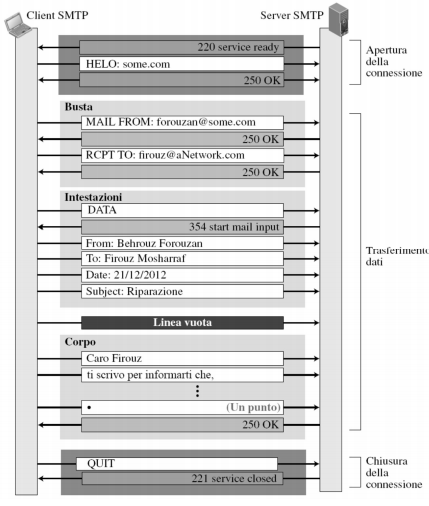
\includegraphics[width=0.8\textwidth]{immagini/SMTP.png}
    \caption*{Fasi della consegna}
\end{figure}

\paragraph{Formato dei messaggi mail}

Il messaggio è suddiviso in intestazioni (header) e corpo (body):\ le intestazioni contengono l'indirizzo del mittente, quello del destinatario, l'argomento del messaggio e alcune altre informazioni, mentre il corpo contiene il messaggio vero e proprio.

\subsubsection{\emph{Multipurpose Internet Mail Extensions (MIME)}}

La posta elettronica ha una struttura molto elementare, ma la sua semplicità comporta che il protocollo possa gestire soltanto messaggi nel formato NVT ASCII a 7 bit.\
Vi sono quindi delle limitazioni; per esempio non possono essere inviati messaggi in lingue che non siano supportate dai caratteri ASCII a 7 bit come per esempio il francese, il tedesco, l'ebraico, il russo, il cinese o il giapponese e non possono essere inviati file binari contenenti audio o video.

Il protocollo MIME (Multipurpose Internet Mail Extensions) è un protocollo supplementare che permette l'invio dei messaggi in formati diversi dall'ASCII.\
Esso agisce lato mittente convertendo tutti i dati in formato non ASCII al formato NVT ASCII e consegnando il risultato al client MTA per l'invio.\
Il messaggio viene ritrasformato al formato originale presso il destinatario.

In conclusione si può pensare al protocollo MIME come a un insieme di funzioni che si occupano di tradurre dati non ASCII in formato NVT ASCII e viceversa.

\paragraph{Intestazione MIME}

Il protocollo MIME definisce cinque tipi di intestazioni specifiche che si aggiungono a quelle originali previste dal protocollo di posta elettronica.

\begin{table}[H]
    \centering
    \begin{tabular}{|p{13cm}|}
        \hline
        Intestazioni della e-mail                                             \\
        \hline
        MIME-Version:\ 1.1                                                    \\
        Content-Type:\ tipo/sottotipo                                         \\
        Content-ID:\ identificatore del messaggio                             \\
        Content-Description:\ spiegazione testuale del contenuto non testuale \\
        \hline
        Corpo della e-mail                                                    \\
        \hline
    \end{tabular}
    \caption*{Intestazioni MIME}
\end{table}

\begin{flushleft}
    \textbf{MIME-version}.\
    In questa intestazione viene dichiarata la versione MIME usata.\
    La versione attuale è la 1.1.

    \textbf{Content-Type}.\
    Intestazione che definisce il tipo di dati nel corpo del messaggio; il tipo del contenuto e il sottotipo sono separati da una barra.\
    A seconda del sottotipo l'intestazione può contenere altri parametri.

    \textbf{Content-Transfer-Encoding}.\
    Definisce il metodo utilizzato per la codifica del messaggio in binario per il trasporto.

    \textbf{Content-ID}.\
    Intestazione che individua univocamente una parte del messaggio in messaggi composti da multiple parti.

    \textbf{Content-Description}.\
    Intestazione che indica se il corpo del messaggio contiene un'immagine, un file audio o un video.
\end{flushleft}

\subsubsection{Message Access Agent:\ i protocolli POP e IMAP}

Il primo e il secondo stadio della trasmissione della posta elettronica utilizzano SMTP, che non è invece impiegato nel terzo stadio essendo un protocollo di tipo push:\ esso ``spinge'' il messaggio dal client al server.\
In altri termini, la direzione della maggior parte dei dati (messaggi) è dal client al server.\
Il terzo stadio richiede invece un protocollo di tipo pull:\ il client deve ``tirare'' i messaggi dal server; in questo caso la direzione della maggior parte dei dati è dal server al client.\
Il terzo stadio utilizza dunque un \emph{Message Access Agent}.

Attualmente si utilizzano due protocolli per l'accesso ai messaggi:\ POP3 (Post Office Protocol, versione 3) e IMAP4 (Internet Mail Access Protocol, versione 4).

\paragraph{\emph{POP3}}
Il protocollo Post Office Protocol versione 3 è molto semplice ma ha funzionalità limitate.\
Il software client POP3 è installato sul computer del destinatario, mentre il software POP3 server viene installato sul server di posta.\
L'accesso alla porta avviene quando il client scarica i messaggi (le e-mail) dalla propria casella di posta che si trova sul server.\
Il client apre una connessione TCP verso il server sulla porta nota 110, quindi invia il proprio nome utente e relativa password per accedere alla casella di posta.\
A questo punto l'utente può richiedere la lista dei messaggi presenti e prelevarli, uno alla volta.

Il protocollo POP3 ha due modalità:\ delete (elimina) e keep (conserva).\
Nella prima i messaggi sono automaticamente eliminati dalla mailbox dopo il prelievo; nella seconda, invece, vengono conservati.

\paragraph{\emph{IMAP4}}
Un altro protocollo di accesso alla posta è l'Internet Mail Access Protocol versione 4 (IMAP4).\
Questo protocollo è simile al POP3 ma ha più funzionalità:\ è più potente e complesso.

POP3 è limitato sotto vari aspetti.\
Non consente all'utente di organizzare la propria posta e di gestire più cartelle sul server.\
POP3, inoltre, non consente all'utente di controllare parte del contenuto del messaggio prima del suo prelievo completo.\
IMAP4, invece, fornisce varie funzionalità aggiuntive quali:
\begin{itemize}
    \item controllare l'intestazione dei messaggi prima del prelievo;
    \item ricercare una stringa specifica nei messaggi prima del prelievo;
    \item prelevare i messaggi in modo parziale.\
          Una funzionalità particolarmente utile quando vi sono limitazioni di banda e i messaggi comprendono contenuti multimediali particolarmente voluminosi;
    \item creare, cancellare o rinominare le mailbox sul server di posta;
    \item creare una gerarchia di cartelle all'interno della mailbox sul server a scopo di archiviazione.
\end{itemize}

\subsection{Il DNS (Domain Name System)}

I dispositivi connessi in rete vengono individuati dai protocolli TCP/IP mediante il loro indirizzo IP; gli utenti, però, preferiscono usare nomi piuttosto che indirizzi numerici.\
Per questo motivo è necessario un sistema che associ un indirizzo IP ad ogni nome.\
Si tratta di una situazione analoga alla rete telefonica, che è progettata per utilizzare dei numeri di telefono, non dei nomi.

Vista la dimensione di Internet, un sistema centralizzato non potrebbe gestire tutte le associazioni necessarie.\
Inoltre se tale sistema centralizzato si dovesse guastare, collasserebbe l'intera rete.\
La soluzione attualmente adottata consiste nel suddividere questa enorme massa di informazioni e distribuire le varie parti ottenute su calcolatori sparsi nel mondo.\
L'host che ha bisogno di associare un indirizzo a un nome, o viceversa, contatta il calcolatore più vicino e gli invia una richiesta opportuna.\
Questo metodo viene usato dal Domain Name System (DNS).

Un utente vuole utilizzare un client per il trasferimento di file per accedere al file server corrispondente, in esecuzione su un host remoto.\
L'utente conosce solo il nome simbolico del file server, per esempio \emph{afilesource.com}.\
Lo stack TCP/IP ha bisogno invece dell'indirizzo IP del file server per stabilire una connessione.

I sei passi seguenti consentono di associare l'indirizzo IP al nome simbolico dell'host:

\begin{enumerate}
    \item l'utente comunica il nome dell'host al client di trasferimento file;
    \item il client di trasferimento file trasmette il nome dell'host al client DNS;
    \item qualsiasi computer, una volta avviato, conosce l'indirizzo IP di un server DNS.\ Il client DNS invia dunque un messaggio al server DNS contenente la richiesta di traduzione del nome simbolico del file server.
    \item il server DNS risponde con l'indirizzo IP del file server desiderato;
    \item il client DNS comunica l'indirizzo IP al client di trasferimento file;
    \item il client di trasferimento file utilizza ora l'indirizzo IP ricevuto per accedere al file server.
\end{enumerate}

Si noti che anche se lo scopo è quello di scambiare un file, prima che questo sia possibile è necessario sfruttare un altro servizio presente su Internet, attraverso l'interazione tra un client e un server DNS.

\subsubsection{\emph{Spazio dei nomi}}

Al fine di evitare ogni ambiguità è necessario definire uno spazio dei possibili nomi da assegnare ai calcolatori connessi in rete.\
In questo spazio si deve poter associare in modo univoco un nome a un indirizzo, in modo tale che anche il nome individui senza ambiguità un calcolatore.\
Vi sono due modi possibili per organizzare tale spazio:\ spazio con struttura piatta e spazio con struttura gerarchica.\
In uno \emph{spazio dei nomi con struttura piatta} viene associato un nome differente a ciascun indirizzo; ogni nome è quindi una sequenza di caratteri senza alcuna struttura interna.\
Due nomi possono avere una sottosequenza di caratteri in comune, ma il fatto che l'abbiano o meno non ha alcuna ulteriore implicazione o significato.\
Il problema fondamentale di questo tipo di spazio, in una rete grande come Internet, è la necessità che esso sia controllato a livello centrale per evitare ambiguità e duplicazioni.\
In uno \emph{spazio dei nomi gerarchico} ogni nome è composto da diverse parti:\ la prima può definire la natura dell'organizzazione, la seconda il suo nome, la terza i vari dipartimenti all'interno dell'organizzazione e così via.\
Con uno spazio di questo tipo gli enti o società che si occupano di assegnare e controllare i nomi possono avere una struttura decentralizzata:\ l'ente centrale si occuperà della parte di nome che corrisponde alla natura dell'organizzazione e alla sua denominazione, per la parte restante del nome la responsabilità di gestione può essere demandata all'organizzazione stessa.\
Questa può aggiungere prefissi o suffissi al nome per individuare i suoi host, o più in generale le sue risorse, senza preoccuparsi di eventuali coincidenze con i prefissi scelti da altre organizzazioni.\
Anche se due diverse organizzazioni scegliessero il medesimo prefisso per alcuni dei loro host, la cosa non creerebbe problemi, perché gli indirizzi sarebbero comunque diversi nella parte riguardante il tipo e la denominazione dell'organizzazione.

\paragraph{\emph{Spazio dei nomi di dominio}} Lo spazio dei nomi di dominio (domain name space) è alla base della costruzione dello spazio dei nomi con struttura gerarchica.\
In questo schema i nomi hanno una struttura ad albero con la radice in cima e un numero di livelli variabile tra 0 (la radice) e 127.

\paragraph{Etichette} Ogni nodo è individuato da un'etichetta (label) costituita al più da 63 caratteri.\
Alla radice (root) è associata un'etichetta vuota, a tutti i nodi collegati a un medesimo nodo da rami diversi sono associate etichette diverse, garantendo così l'univocità dei nomi di dominio.

\paragraph{Nomi di dominio} Ogni nodo dell'albero ha un nome di dominio (domain name), ovvero una sequenza di etichette separate da punti (.), che lette da sinistra a destra forniscono tutte le etichette associate ai vari nodi a partire da quello in questione fino alla radice.\
L'ultima etichetta è quella della radice, la stringa nulla, quindi tutti i nomi di dominio terminano con un punto.\
Tutte le etichette che si trovano immediatamente sotto la radice vengono definite \emph{top-level} (di livello più alto) e quindi si parlerà di domini top-level.
Una sequenza di etichette che termina con una stringa nulla è detta \emph{nome di dominio pienamente qualificato} o \emph{FQDN} (Fully Qualified Domain Name).\
Si osservi che il nome termina con una stringa nulla e quindi l'ultimo carattere risulta essere un punto (.).\
Una sequenza di etichette che non termina con una stringa nulla è detta \emph{nome di dominio parzialmente qualificato} o \emph{PQDN} (Partially Qualified Domain Name).\
Un PQDN, quindi, inizia da un nodo ma non raggiunge la radice; esso viene usato quando il nome da risolvere e il client appartengono allo stesso dominio di livello superiore.\
In questo caso, infatti, il protocollo atto alla risoluzione del nome può aggiungere automaticamente la parte mancante, detta suffisso, al fine di ottenere un FDQN.

\paragraph{\emph{Domini}} Un dominio (domain) è un sottoalbero dello spazio dei nomi di dominio che viene identificato dal nome di dominio del nodo in cima al sottoalbero; si osservi che un dominio può essere suddiviso in ulteriori domini, detti talvolta sottodomini.

\paragraph{\emph{Informazioni degli spazi di dominio}} Le informazioni contenute nello spazio dei nomi di dominio devono essere memorizzate in un dispositivo fisico.\
Salvare questa enorme mole di dati su un solo computer sarebbe allo stesso tempo inaffidabile, in quanto il computer potrebbe guastarsi, e inefficiente, poiché per ottenere informazioni relative ai nomi di dominio tutti i calcolatori della rete mondiale dovrebbero rivolgersi a una stessa macchina.\
È quindi necessario trovare una soluzione alternativa.

\subsubsection{\emph{Gerarchie dei Name Server}}

Il problema appena posto è stato risolto ripartendo le informazioni relative ai nomi di dominio tra diversi calcolatori detti \emph{server DNS} o anche \emph{name server}.\
L'intero spazio è stato suddiviso in diversi domini differenziati al primo livello dell'albero; in altri termini la radice resta comune e a ogni nodo di primo livello è stato associato un dominio.\
Poiché i domini così ottenuti continuano a essere molto vasti, essi sono stati suddivisi in domini più piccoli, detti \emph{sottodomini}.\
Ogni server è responsabile di un dominio o di un sottodominio:\ vi è quindi una gerarchia di server che implementa la gerarchia di nomi.

\paragraph{\emph{Zone}}

Poiché non è possibile memorizzare la gerarchia completa dei nomi di dominio su un singolo server, questa viene suddivisa fra numerosi server.\
Una \emph{zona} è tutto ciò di cui è responsabile un server.\
Si può definire una zona come una parte contigua dell'intero albero.\
Se un server accetta tutte le responsabilità per un dominio e non effettua suddivisioni in sottodomini, allora la zona e il dominio coincidono.\
Ogni server ha un database, detto \emph{file di zona}, in cui vengono elencate tutte le informazioni relative ai nodi presenti nella sua zona di competenza.\
Se, invece, il server suddivide il proprio dominio in sottodomini, allora la zona e il dominio si differenziano.\
In questo caso il server ha delegato una parte della sua autorità ad uno o più altri server.

Le informazioni relative ai nodi nei sottodomini sono immagazzinate nei server di livello più basso e il server originario si limita a gestire i riferimenti a questi server di livello inferiore.\
Ovviamente il server originario non risulta totalmente privo di responsabilità:\ a esso è ancora associata una zona, ma le informazioni dettagliate sui nodi di tale zona sono immagazzinate nei server di livello più basso.

\paragraph{\emph{Server radice}}

Un server radice (\emph{root server}) è un server che ha per zona l'intero albero.\
Solitamente i root server delegano la loro responsabilità ad altri server e si limitano a immagazzinare riferimenti relativi a questi server.\
Attualmente vi sono vari server radice distribuiti sulla rete Internet, ciascuno dei quali gestisce l'intero spazio dei nomi di dominio.\
I root server sono fisicamente distribuiti in tutto il mondo.

\subsubsection{\emph{Server primari e secondari}}

I server DNS possono essere primari o secondari.\
Un \emph{server primario} possiede un file relativo alla zona sotto la sua responsabilità (e autorità):\ la creazione, la gestione e l'aggiornamento del file di zona sono di sua competenza.\
Il file di zona è memorizzato nel suo disco locale.

Un \emph{server secondario} riceve tutte le informazioni relative a una certa zona da un altro server, primario o secondario, e le memorizza in un file nel suo disco.\
I server secondari non creano né aggiornano i file di zona; sono i server primari che effettuano queste operazioni e poi trasmettono il nuovo file ai server secondari.

I server primari e secondari hanno entrambi la medesima autorità sulla zona di loro competenza (spesso si dice che sono ``autorevoli'' o ``autoritativi''), in altri termini sono allo stesso livello di autorità; ma l'introduzione di un server secondario porta a una duplicazione, che può risultare utile in caso di guasti al server primario.\
Si osservi anche che un certo server può fungere da primario per una certa zona e da secondario per un'altra; gli aggettivi primario e secondario, quindi, vanno riferiti alla zona a cui ci si riferisce.

\subsubsection{\emph{Server DNS nella rete Internet}}

Il protocollo DNS può essere utilizzato su diverse piattaforme; nel caso di Internet lo spazio dei nomi di dominio (l'albero) è stato originariamente diviso in tre parti:\emph{domini generici}, \emph{nazionali} e \emph{inversi}.\
Tuttavia, a causa della rapidissima espansione di Internet, è divenuto troppo complesso tenere traccia dei domini inversi, che potevano essere utilizzati per trovare il nome dell'host corrispondente partendo da un indirizzo IP.\
I domini inversi sono oggi obsoleti.

\paragraph{\emph{Domini generici}}

I \textbf{domini generici} suddividono gli host in base al loro scopo generale; ogni nodo dell'albero definisce un dominio che non è altro che un indice nel database dello spazio dei nomi di dominio.

\paragraph{\emph{Domini nazionali}}

Il formato dei \textbf{domini nazionali} prevede un'etichetta di primo livello costituita da abbreviazioni formate da due caratteri e che individuano una nazione.\
Il significato della seconda etichetta varia da nazione a nazione:\ negli Stati Uniti serve a individuare lo Stato dell'Unione.

\subsubsection{\emph{Risoluzione}}

Il processo che permette di associare un indirizzo IP a un nome è detto \emph{risoluzione} di un nome (address resolution).\
Il DNS è progettato come applicazione client/server.\
Un host che voglia associare un nome a un indirizzo IP (o viceversa, quando è possibile) si rivolge a un programma client DNS che è detto \textbf{resolver} (risolutore).\
Il resolver invia un'opportuna richiesta al server DNS più vicino; questi, se ha l'informazione, comunica l'indirizzo o il nome cercato al resolver, altrimenti o si rivolge a un altro server o comunica al resolver l'indirizzo di un altro server a cui fare riferimento.\
Ricevuta la risposta, il resolver l'analizza per accertarsi che non contenga errori e trasmette il risultato al processo che aveva richiesto la risoluzione.\
La modalità di svolgimento della \textbf{risoluzione} può essere \textbf{ricorsiva} o \textbf{iterativa}.

\paragraph{\emph{Risoluzione ricorsiva}}

Supponiamo che un programma applicativo eseguito su un host di nome \emph{pads.cs.unibo.it} voglia trovare l'indirizzo IP di un altro host chiamato \emph{engineering.mcgraw-hill.com} a cui inviare un messaggio.\
L'host sorgente è connesso alla rete dell'Università di Bologna, mentre l'host destinatario è connesso alla rete McGraw-Hill.

Il programma applicativo sull'host sorgente chiede al resolver (il client) DNS l'indirizzo IP dell'host destinatario.\
Il resolver, che non conosce tale indirizzo, invia una query al server DNS locale fornito dall'università.\
Ipotizziamo che anche questo server non conosca l'indirizzo IP dell'host destinatario.\
Invia quindi la query a un server DNS radice, il cui indirizzo IP si suppone noto a questo server DNS locale.\
I server radice solitamente non mantengono le associazioni fra nomi e indirizzi IP, ma devono conoscere almeno un server per ogni dominio top-level.\
La query viene quindi inviata a questo server di dominio top-level.\
Ipotizziamo che questo server non conosca l'associazione nome/indirizzo IP di questo particolare destinatario, ma conosca l'indirizzo IP del server DNS locale dell'azienda McGraw-Hill.\
La query viene così inviata a questo nuovo server che conosce l'indirizzo IP dell'host destinatario.\
L'indirizzo IP viene ora inviato al server DNS top-level, quindi al server radice, poi al server DNS dell'università che potrebbe memorizzarlo nella propria cache per eventuali richieste future, ed infine viene restituito all'host sorgente.

\paragraph{\emph{Risoluzione iterativa}}

Nel caso della risoluzione iterativa ogni server che non conosce la risposta alla domanda del client risponde con l'indirizzo di un altro server in grado di risolvere il problema.\
Solitamente la risoluzione iterativa ha luogo fra due server locali, il resolver originale riceve la risposta finale dal server locale.

\paragraph{\emph{Caching}}

Un server, ogni volta che riceve una richiesta di risoluzione per un nome che non si trova all'interno del suo dominio, deve cercare nel proprio database l'indirizzo di un altro server al quale eventualmente inoltrare la richiesta.\
Ridurre questo tempo di ricerca significa aumentare l'efficienza.\
Questo avviene per mezzo di un meccanismo detto \emph{caching}.\
Quando un server si rivolge a un secondo server per la risoluzione di un indirizzo archivia la sua risposta in una memoria temporanea, o memoria cache, al fine di poter usare questa informazione per successive richieste di risoluzione.\
Quando un server riceve una richiesta e la risposta è già presente in memoria cache, questa viene inviata al client segnalando però che si tratta di una risposta non autorevole (\emph{unauthoritive}).

La tecnica del caching permette di velocizzare le procedure di risoluzione, ma può anche generare problemi; infatti se un server conservasse troppo a lungo un'informazione nella sua memoria cache, correrebbe il rischio di inviare ai client informazioni obsolete.\
Per evitare questi problemi, i server autorevoli aggiungono alle informazioni da loro trasmesse un campo detto \emph{tempo residuo} (time to live, TTL), che stabilisce per quanti secondi il server ricevente può conservare l'informazione nella sua memoria cache.\
Trascorso questo tempo la corrispondenza non è più valida, le informazioni vengono eliminate dalla memoria cache ed eventuali nuove interrogazioni verranno trasmesse al server autorevole.\
Il DNS richiede che ogni server mantenga un contatore TTL per ciascuna associazione memorizzata.\
La memoria cache deve essere poi controllata periodicamente per eliminare le associazioni con TTL scaduto.

\subsubsection{\emph{Record di risorsa}}

A ogni nome di dominio (un nodo dell'albero dello spazio dei nomi) è associato un record di risorsa.\
Il database del server dei nomi non è altro che una collezione di record risorsa che vengono inviati al client che ne fa richiesta.\
Un record risorsa è formato da cinque campi:

\begin{center}
    (\textbf{Nome di dominio}, \textbf{Tipo}, \textbf{Classe}, \textbf{TTL}, \textbf{Valore})
\end{center}

Il campo \emph{nome di dominio} identifica il record risorsa.\
Il campo \emph{valore} contiene l'informazione memorizzata relativa al nome di dominio.\
Il campo \emph{TTL} indica il numero di secondi per cui l'informazione deve essere ritenuta valida.\
Il campo \emph{classe} definisce il tipo di rete:\ in questo contesto si è esclusivamente interessati alla classe IN (Internet).\
Il \emph{tipo} definisce infine come interpretare il campo valore.

\begin{table}[H]
    \centering
    \begin{tabular}{|c|p{11 cm}|}
        \hline
        \emph{Tipo} & \emph{Interpretazione del campo valore}                                   \\
        \hline\hline
        A           & Indirizzo IPv4 a 32 bit                                                   \\
        \hline
        NS          & Identifica i server autoritativi in una zona                              \\
        \hline
        CNAME       & Indica che un nome di dominio è un alias per il nome di dominio ufficiale \\
        \hline
        SOA         & Specifica una serie di informazioni autoritative riguardo una zona        \\
        \hline
        MX          & Indica il server di posta del dominio                                     \\
        \hline
        AAAA        & Indirizzo IPv6                                                            \\
        \hline
    \end{tabular}
    \caption*{Tipi di record}
\end{table}

\subsubsection{\emph{Messaggi DNS}}

I messaggi DNS sono di due tipi, \emph{interrogazione} (\emph{query}) e \emph{risposta} (\emph{response}), e hanno lo stesso formato.

Il campo identificatore è utilizzato dal client per associare la risposta all'interrogazione.\
Il campo flag indica se si tratta di un messaggio di richiesta o di risposta; è utilizzato anche per segnalare eventuali errori.\
I quattro campi successivi nell'intestazione definiscono il numero di ciascun tipo di record nel messaggio.\
La sezione richiesta, che è inclusa nell'interrogazione ed è ripetuta nel messaggio di risposta, consiste di uno o più record di richiesta.\
La sezione risposta, presente esclusivamente nei messaggi di risposta, consiste di uno o più record di risorsa.\
La sezione autorevole fornisce informazioni (nome di dominio) di uno o più server autorevoli per l'interrogazione.\
La sezione supplementare fornisce informazioni addizionali che potrebbero essere utili al risolutore.

\begin{table}[H]
    \centering
    \begin{tabular}{|m{15em}|m{15em}|}
        \hline
        Identificazione                                                            & Flag                                                                     \\
        \hline
        Numero dei record di richiesta                                             & Numero dei record di risposta (tutti 0 nei messaggi di interrogazione)   \\
        \hline
        Numero dei record di autoritativi (tutti 0 nei messaggi di interrogazione) & Numero dei record supplementari (tutti 0 nei messaggi di interrogazione) \\
        \hline
        \multicolumn{2}{|c|}{Sezione richiesta}                                                                                                               \\
        \hline
        \multicolumn{2}{|c|}{Sezione risposta (record risorsa)}                                                                                               \\
        \hline
        \multicolumn{2}{|c|}{Sezione autoritativa}                                                                                                            \\
        \hline
        \multicolumn{2}{|c|}{Sezione supplementare}                                                                                                           \\
        \hline
    \end{tabular}
    \caption*{Struttura dei messaggi DNS}
\end{table}

\subsubsection{\emph{Protocollo di livello trasporto}}

Il sistema DNS può usare sia il protocollo UDP che quello TCP; in entrambi i casi il server usa il numero di porta noto 53.\
Il protocollo UDP viene usato quando la dimensione del messaggio di risposta è inferiore a 512 byte, perché molto spesso i datagrammi utente UDP non possono superare i 512 byte di dimensione massima.\
In caso contrario viene usato il protocollo TCP.

\subsection{FTP}

FTP (File Transfer Protocol) è il protocollo standard offerto da TCP/IP per la copia di file da un host a un altro.

\begin{itemize}
    \item Servizio diverso dall'accesso condiviso on-line (accesso simultaneo da parte di più programmi ad un singolo file)
    \item Trasferimento file:\ si ottiene una copia locale (si effettuano modifiche in locale) ed eventuale trasferimento del file modificato in remoto.
\end{itemize}
Sebbene il trasferimento di un file possa sembrare un'operazione semplice, vi sono, in realtà, numerosi problemi ai quali bisogna prestare attenzione:\ i due sistemi coinvolti, per esempio, possono adottare convenzioni differenti per la denominazione dei file, oppure gestire in modo differente la struttura delle directory.\
Problemi di questo tipo vengono risolti in modo semplice ed elegante dal protocollo FTP.

FTP fornisce funzionalità aggiuntive rispetto al semplice trasferimento file:

\begin{itemize}
    \item accesso interattivo:\ l'utente può navigare e cambiare/modificare l'albero di directory nel file system remoto;
    \item specifica del formato dei dati da trasferire (es.\ file di testo o file binari);
    \item autenticazione:\ il client può specificare login e password.
\end{itemize}

Sebbene sia possibile trasferire file con HTTP, FTP rimane la scelta migliore per trasferire file voluminosi.

Il client ha tre componenti:\ interfaccia utente, processo di controllo e processo di trasferimento dati.\
Il server ha, invece, due sole componenti:\ processo di controllo e processo di trasferimento dati.\
La connessione di controllo viene realizzata tra i due processi di controllo e quella per lo scambio dei dati tra i due processi relativi.

FTP usa la connessione di controllo per permettere a client e server di coordinare l'uso delle porte assegnate dinamicamente \textbf{per il trasferimento dati}.\
La separazione del trasferimento dei dati e dei comandi rende il controllo FTP piuttosto efficiente:\ la connessione che si occupa delle informazioni di controllo può usare regole molto semplici, così che lo scambio di informazioni si riduce allo scambio di una riga di comando (o di risposta) per ogni interazione.\
La connessione che si occupa dello scambio di dati, invece, deve fare uso di regole più complesse a causa della varietà delle informazioni scambiate.

Inoltre, FTP è un protocollo \emph{stateful}:\ il server deve tenere traccia dello stato dell'utente (connessione di controllo associata ad un account, directory attuale, ecc.).

\subsubsection{\emph{Durata delle due connessioni}}

Le due connessioni in FTP hanno durate differenti.\
La connessione di controllo rimane aperta durante l'intera sessione FTP interattiva.\
La connessione dati viene aperta e chiusa per ciascun trasferimento file:\ viene aperta a ogni comando che comporta il trasferimento di uno o più file, per essere chiusa al termine del trasferimento.\
Quando un utente inizia una sessione FTP viene aperta la sessione di controllo; mentre questa è aperta, la connessione dati può essere aperta e chiusa più volte se vengono trasferiti più file.\
Il protocollo FTP usa due porte TCP note:\ la porta 21 è usata per la connessione di controllo e la 20 per lo scambio dei dati.

\subsubsection{\emph{Connessione di controllo}}

\begin{enumerate}
    \item Il client FTP contatta il server FTP alla porta 21
    \item Il client ottiene l'autorizzazione sulla connessione di controllo
    \item Il client invia i comandi sulla connessione di controllo (es.\
          cambio di directory, invio file, ecc.)
\end{enumerate}
La connessione di controllo è \emph{persistente}

Il protocollo FTP usa lo stesso approccio usato da TELNET:\ la comunicazione attraverso la connessione di controllo avviene per mezzo di caratteri con una codifica standard chiamata NVT ASCII, sia per i comandi sia per le risposte.\
Pur nella sua semplicità questo metodo è perfettamente adeguato perché l'interazione avviene mediante l'invio di un comando o di una  risposta alla volta.\
Ogni riga termina con la coppia di caratteri ritorno carrello e fine linea.

Durante questa connessione di controllo i comandi vengono inviati dal client al server e le risposte vengono inviate dal server al client.\
I comandi sono inviati al processo di controllo del client FTP sotto forma di caratteri ASCII maiuscoli e possono opzionalmente essere seguiti da un argomento.

Ogni comando FTP genera almeno una risposta; le risposte sono composte da due parti:\ un numero di tre cifre e un testo.\
La parte numerica costituisce il codice della risposta, quella di testo contiene i parametri necessari o infromazioni supplementari.\
La prima cifra fornisce lo stato del comando.\
La seconda cifra definisce l'area alla quale si applica lo stato.\
La terza cifra fornisce informazioni supplementari.

\pagebreak
\subsubsection{\emph{Connessione per lo scambio dei dati}}

Per creare la connessione TCP per il trasferimento dati sono possibili due modalità:

\begin{itemize}
    \item \textbf{Active mode}:
          \begin{enumerate}
              \item Il client, non il server, effettua un'apertura passiva usando una porta effimera (rimarrà in attesa di connessione); ciò viene fatto dal client perché è tale processo che invierà i 				comandi per il trasferimento dei file.
              \item Il client invia questo numero di porta al server per mezzo del comando PORT.
              \item Il server, ricevuto il numero di porta, effettua un'apertura attiva (aprirà la connessione) usando la porta nota 20 e quella effimera segnalata dal client.
          \end{enumerate}
    \item \textbf{Passive mode}:\ il client chiede al server di mettersi in ascolto su una porta per una connessione dati tramite il comando PASV, ottiene questo numero di porta dal server e lo usa per aprire la connessione con il server (porta 20 ma non necessariamente)
          \begin{itemize}
              \item Il server fa un'apertura passiva (si mette in ascolto di richieste di connessione su una porta), il client fa un'apertura attiva.
          \end{itemize}
\end{itemize}
La connessione dati è \emph{non persistente}, una per ciascun trasferimento.

\paragraph{Comunicazione lungo la connessione per lo scambio dei dati}

La connessione per lo scambio dei dati ha caratteristiche e scopi diversi da quella di controllo.\
Lo scopo ultimo è il trasferimento di file:\ il client deve definire il tipo del file, la struttura dei dati e la modalità di trasmissione al fine di risolvere i problemi di eterogeneità tra il client e il server.\
Il trasferimento del file viene preparato mediante uno scambio di informazioni lungo la connessione di controllo.

\paragraph{Trasferimento di file}

Il trasferimento dei file avviene lungo la connessione per lo scambio dei dati sotto il controllo dei comandi trasmessi lungo la connessione di controllo.\
Bisogna ricordare, comunque, che trasferire un file con il protocollo FTP vuol dire effettuare una delle operazioni seguenti:\ copiare un file dal server al client (retrieving di un file), copiare un file dal client al server (storage di un file) e ottenere una lista dei file presenti sul server (listing).

\begin{table}[H]
    \centering
    \begin{tabular}{|l|l|m{16em}|}
        \hline
        \emph{Comando} & \emph{Argomenti}       & \emph{Descrizione}                              \\
        \hline
        ABOR           &                        & Interruzione del comando precedente             \\
        \hline
        CDUP           &                        & Sale di un livello nell'albero delle directory  \\
        \hline
        CWD            & Nome della directory   & Cambia la directory corrente                    \\
        \hline
        DELE           & Nome del file          & Cancella il file                                \\
        \hline
        LIST           & Nome della directory   & Elenca il contenuto della directory             \\
        \hline
        MKD            & Nome della directory   & Crea una nuova directory                        \\
        \hline
        PASS           & Password utente        & Password                                        \\
        \hline
        PASV           &                        & Il server sceglie la porta                      \\
        \hline
        PORT           & Numero di porta        & Il client sceglie la porta                      \\
        \hline
        PWD            &                        & Mostra il nome della directory corrente         \\
        \hline
        QUIT           &                        & Uscita dal sistema                              \\
        \hline
        RETR           & Nome di uno o più file & Trasferisce uno o più file dal server al client \\
        \hline
        RMD            & Nome della directory   & Cancella la directory                           \\
        \hline
        RNTO           & Nome (del nuovo) file  & Cambia il nome del file                         \\
        \hline
        STOR           & Nome di uno o più file & Trasferisce uno o più file dal client al server \\
        \hline
        USER           & Identificativo         & Identificazione dell'utente                     \\
        \hline
    \end{tabular}
    \caption*{Principali comandi FTP}
\end{table}

\begin{table}[H]
    \centering
    \begin{tabular}{|l|m{12em}|l|m{12em}|}
        \hline
        \emph{Codice} & \emph{Descrizione}           & \emph{Codice} & \emph{Descrizione}                                 \\
        \hline
        125           & Connessione dati aperta      & 250           & Azione sul file OK                                 \\
        \hline
        150           & Stato del file OK            & 331           & Nome dell'utente OK, in attesa della password      \\
        \hline
        200           & Comando OK                   & 425           & Non è possibile aprire la connessione dati         \\
        \hline
        220           & Servizio pronto              & 450           & Azione sul file non eseguita; file non disponibile \\
        \hline
        221           & Servizio in chiusura         & 452           & Azione interrotta; spazio insufficiente            \\
        \hline
        225           & Connessione dati aperta      & 500           & Errore di sintassi; comando non riconosciuto       \\
        \hline
        226           & Connessione dati in chiusura & 501           & Errore di sintassi nel parametro o negli argomenti \\
        \hline
        230           & Login dell'utente OK         & 530           & Login dell'utente fallito                          \\
        \hline
    \end{tabular}
    \caption*{Risposte FTP}

\end{table}

\subsubsection{Modalità di trasmissione}

\begin{itemize}
    \item \textbf{Stream mode}:\ FTP invia i dati a TCP con un flusso continuo di bit.
    \item \textbf{Block mode}:\ FTP invia i dati a TCP suddivisi in blocchi.\ Ogni blocco è preceduto da un header.
    \item \textbf{Compressed mode}:\ si trasmette il file compresso.
\end{itemize}

\subsubsection{Conclusione}

FTP può essere usato per amministrare i siti web:\ se è necessario spostare file su server remoti, sui server di un host provider, è possibile usare un client FTP per trasferire i file dalla postazione locale alla postazione in remoto; ovviamente è necessaria l'autenticazione.\
Tuttavia ci sono alcuni server che supportano l'\emph{anonymous FTP}, ovvero una connessione FTP senza autenticazione:

\begin{itemize}
    \item login anonymous;
    \item password guest (o email).
\end{itemize}
Tipicamente consentono di accedere solo ad una parte del file system e permettono solo un subset di operazioni (es.\ no PUT).

Ci sono anche altri protocolli per il trasferimento di file, per esempio basati su SSH.\
Rimanendo su FTP la specifica più sicura e più vicina è l'\emph{FTPS} (securing FTP with TLS):\ meccanismo che può essere usato da client e server FTP per implementare sicurezza e autenticazione usando il protocollo TLS (RFC 2246).

\subsection{Approfondimenti}

\subsubsection{Come migliorare il tempo di caricamento di una pagina agendo a livello di protocollo?}

Con HTTP/1.1:\ i browser instaurano più connessioni TCP in parallelo (tipicamente con un valore massimo di 6 connessioni contemporanee)

\begin{itemize}
    \item Comportamento non equo
    \item Il controllo di congestione è poco efficace
\end{itemize}

\paragraph{HTTP/2}
\begin{enumerate}
    \item \textbf{Multiplexing delle richieste su un'unica connessione TCP}
          \begin{itemize}
              \item \textbf{\emph{Frame}}:\ l'unità di comunicazione in HTTP/2.\ Una sequenza di frame mappa un messaggio HTTP (es.\ un frame può essere un HEADER frame, DATA frame, \dots)
                    \begin{figure}[H]
                        \centering
                        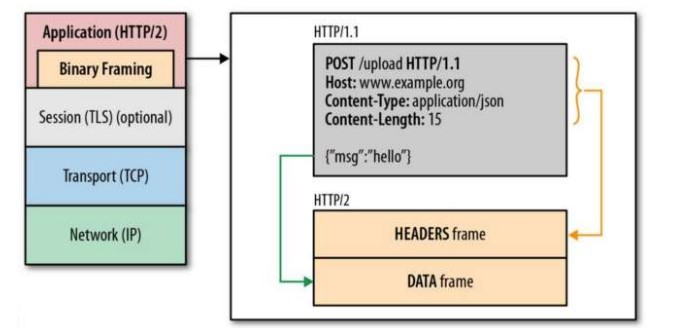
\includegraphics[width = 0.8\textwidth]{immagini/HTTP_2.jpg}
                        \caption*{Frame HTTP/2}
                    \end{figure}
              \item \textbf{\emph{Stream}}:\ un flusso bidirezionale di frame di un'unica connessione TCP, rappresenta una comunicazione richiesta-risposta
              \item Mediante l'astrazione degli stream è possibile effettuare il \textbf{multiplexing delle richieste} (più stream sulla stessa connessione TCP)
                    \begin{figure}[H]
                        \centering
                        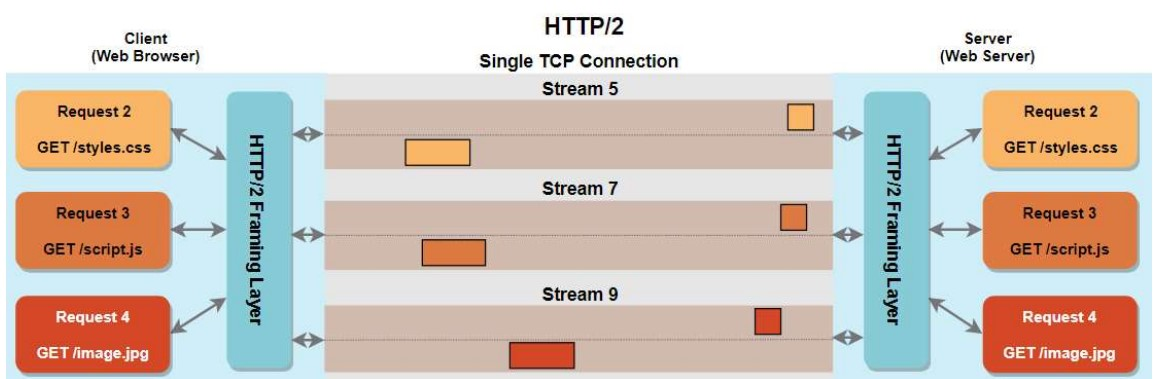
\includegraphics[width = 0.9\textwidth]{immagini/HTTP_2_stream.jpg}
                        \caption*{Multiplexing delle richieste}
                    \end{figure}
          \end{itemize}
    \item \textbf{Definizione delle priorità}:\ è possibile associare ad ogni stream
          \begin{itemize}
              \item un \textbf{peso} che ne indica la priorità
              \item una \textbf{dipendenza} verso altri stream
          \end{itemize}
    \item \textbf{Compressione delle intestazioni}
    \item \textbf{\emph{Server Push}}:\ permette al server di inviare risorse aggiuntive per una singola richiesta da parte del client
\end{enumerate}
HTTP/2 risolve il problema di uso inefficiente di una connessione TCP, in particolare per pagine con tante risorse.

Limite:\ \emph{Head Of Line Blocking}, una perdita (3 ACK/timeout) provoca lo stallo della connessione (e quindi di tutti gli stream).

\begin{figure}[H]
    \centering
    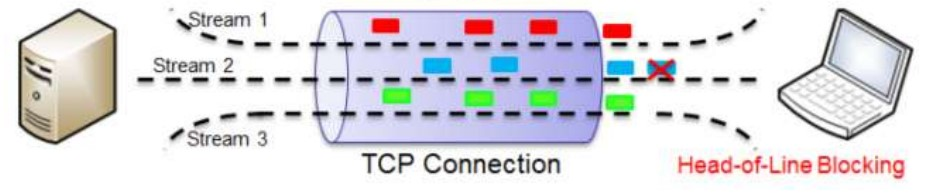
\includegraphics[width = 0.9\textwidth]{immagini/Head_of_line.jpg}
\end{figure}

\paragraph{QUIC}

Protocollo di trasporto che sfrutta UDP.\
Aggiunge:
\begin{itemize}
    \item controllo del flusso e della congestione;
    \item rilevazione delle perdite e ritrasmissione.
\end{itemize}
Astrazione dello stream gestito a livello di trasporto.\
Gli stream sono indipendenti tra loro, la perdita o rallentamento di uno stream non influisce sul progredire degli altri streams.

\paragraph{HTTP/3}

\begin{itemize}
    \item Evoluzione di HTTP/2 che usa i servizi di QUIC
    \item Mantiene la semantica di HTTP/2
    \item Gli stream non sono trasparenti al livello di trasporto
\end{itemize}

\section{Paradigma peer-to-peer}

Il paradigma client/server è stato analizzato nella prima parte di questo capitolo; nei paragrafi precedenti si sono descritte alcune applicazioni client{\slash}server standard.\
In questo paragrafo si analizza il paradigma peer-to-peer (P2P).\
Il primo esempio di condivisione di file P2P risale al 1987 quando Wayne Bell creò WWIVnet, la componente di rete del software WWIV (World War Four).\
Nel luglio del 1999, Ian Clarke progettò Freenet, una struttura decentralizzata e resistente alla censura per l'immagazzinamento e la diffusione di informazioni.\
Freenet ha l'obiettivo, per mezzo di un'architettura P2P, di fornire libertà di parola con forte protezione dell'aninomato.

Il paradigma P2P divenne molto popolare con Napster (1999-2001), un servizio di condivisione di file musicali creato da Shawn Fanning.\
Sebbene la copia e la diffusione non autorizzata di file musicali da parte degli utenti abbia portato a una condanna per violazione dei diritti di copyright costringendo Napster alla chiusura, esso preparò il terreno per i meccanismi di condivisione dei file P2P che apparvero successivamente.\
Il rilascio della prima versione di Gnutella avvenne nel marzo dell'anno 2000.\
Venne seguita da FastTrack (usato da Kazaa), BitTorrent, WinMX e GNUnet rispettivamente in marzo, aprile, maggio e novembre del 2001.

\subsection{Reti P2P}

Gli utenti Internet che intendono condividere le proprie risorse divengono ``\textbf{peer}'' (pari) e formano una rete.
\begin{itemize}
    \item Tutti i nodi (peer) hanno la stessa importanza (in linea di principio):\ nodi indipendenti (autonomi) e localizzati ai bordi (edge) di Internet.
    \item Sistemi altamente distribuiti:\ il numero di nodi può essere dell’ordine delle centinaia di migliaia.
\end{itemize}
Quando uno dei peer nella rete ha un file (per esempio audio o video) da condividere, lo rende disponibile agli altri.\
Chi è interessato può connettersi al computer dove il file è memorizzato e prelevarlo; una volta prelevato, lo può a sua volta rendere disponibile ad altri peer.\
Via via che altri peer entrano a far parte della rete e prelevano il file, il gruppo ha a disposizione sempre più copie.\
Poiché il gruppo di peer può crescere e ridursi dinamicamente, il problema è come poter traccia della disponibilità dei vari file tra i peer.\
Per risolvere questo problema è necessario prima suddividere le reti P2P in due categorie:\ centralizzate e decentralizzate.

\subsubsection{\emph{Reti centralizzate}}
In una rete P2P \emph{centralizzata}, il sistema di directory - ovvero l'elenco dei peer e delle risorse condivise - utilizza il paradigma client/server, ma la memorizzazione e lo scaricamento dei file avvengono usando il paradigma P2P.\
Per questa ragione le reti centralizzate P2P sono a voltre chiamate \emph{reti P2P ibride}.\
Napster è stato un esempio di rete P2P centralizzata.\
In questo tipo di rete, un peer si registra per prima cosa presso un server centrale, al quale fornisce il proprio indirizzo IP e un elenco di file che vuole condividere.\
Per evitare il collasso del sistema, Napster utilizzava numerosi server per questo scopo.

Un peer alla ricerca di un particolare file, invia una richiesta a un server centrale.\
Questo ricerca nella propria directory e rispode con l'indirizzo IP dei nodi che hanno una copia del file.\
Il peer contatta quindi uno (o più) dei nodi e preleva il file.\
La directory è costantemente aggiornata per tenere traccia dei nodi che entrano o escono dalla rete.

Nelle reti centralizzate la gestione del sistema di directory è piuttosto semplice ma presenta vari inconvenienti.\
L'accesso alla directory può generare un traffico enorme e rallentare tutto il sistema.\
I server centrali sono vulnerabili agli attacchi e, se dovessero subire danni, l'intero sistema collasserebbe.\
Napster perse la causa relativa alla violazione del copyright proprio a causa della componente centrale del sistema, che fu ritenuta direttamente responsabile delle attività illegali condotte dagli utenti, e fu costretto a chiudere nel luglio del 2001.

\subsubsection{\emph{Reti decentralizzate}}

Una rete P2P \emph{decentralizzata} non utilizza un sistema directory centralizzato.\
Con questo modello i peer si organizzano formando un \emph{overlay network}, ovvero una rete logica soprastante alla rete fisica utilizzata per organizzare i peer.\
A seconda di come sono collegati i nodi della rete sovrastante (la modalità di organizzazione), una rete P2P decentralizzata si classifica in strutturata o non strutturata.

\paragraph{\emph{Reti non strutturate}}

I nodi in una rete \emph{non strutturata} sono collegati tra loro in modo casuale.\
Una ricerca in una rete P2P non strutturata non è molto efficiente poiché una qualsiasi interrogazione (ad esempio proprio per trovare un file) deve essere inviata in \emph{flooding} (ogni nodo deve inviare la richiesta a tutti gli altri nodi con cui ha un collegamento diretto) a tutta la rete:\ questo produce un volume di traffico rilevante e, nonostante questo, la ricerca potrebbe avere esito negativo.\
Tuttavia, l'aggiunta o la rimozione dei nodi è un'operazione semplice e poco costosa; tali reti sono infatti adatte per gestire nodi con un comportamento fortemente transiente (tassi di join/leave elevati).\
Esempi di questo tipo di rete sono Gnutella e Freenet.

La rete Gnutella è un esempio di rete P2P decentralizzata e non strutturata.\
Non è strutturata nel senso che il meccanismo di directory è distribuito tra nodi.\
Quando il nodo A desidera accedere a un oggetto (per esempio un file) contatta uno dei suoi vicini, uno qualsiasi dei nodi con cui è collegato nella rete di overlay.\
Il nodo A invia quindi un messaggio di richiesta (query) al suo vicino W.\
La richiesta contiene le informazioni necessarie per identificare l'oggetto richiesto (per esempio il nome del file).\
Se il nodo W conosce l'indirizzo del nodo X che possiede l'oggetto, trasmette un messaggio di risposta (response) che contiene l'indirizzo del nodo X.\
Il nodo A può ora utilizzare un protocollo di trasferimento come HTTP per ottenere una copia dell'oggetto dal nodo X.\
Se il nodo W non conosce l'indirizzo del nodo X, invia in flooding la richiesta di A a tutti i suoi nodi vicini.\
Alla fine uno dei nodi della rete risponderà al messaggio di interrogazione, e il nodo A potrà accedere al nodo X.\
Sebbene in Gnutella il meccanismo di flooding sia implementato in modo da evitare un traffico eccessivo, una delle ragioni per cui Gnutella è difficilmente scalabile è proprio per l'impiego di questa tecnica.

Uno dei problemi non ancora affrontati è come possa il nodo A conoscere l'indirizzo di almeno un vicino.\
Questo viene effettuato nella cosiddetta fase di bootstrap (accesso iniziale del client alla rete P2P) attraverso varie strategie.\
Nella più semplice il software include un elenco di nodi (peer) che il nodo A può memorizzare immediatamente come vicini.

\paragraph{Copertura gerarchica}

\begin{itemize}
    \item Cerca di combinare il ``meglio'' delle reti centralizzate e del query flooding:
          \begin{itemize}
              \item no server con tutti i contenuti (solo ``bootstrap servers'');
              \item i peer non sono tutti uguali (esistono i group leader).
          \end{itemize}
    \item Ogni peer
          \begin{itemize}
              \item è group leader (se ``potente'' in banda o risorse)
              \item oppure viene assegnato a un group leader
          \end{itemize}
    \item Connessioni TCP
          \begin{itemize}
              \item tra peer e il suo group leader
              \item tra (alcune) coppie di group leader
          \end{itemize}
    \item Group leader tiene traccia del contenuto dei suoi ``figli''
          \begin{itemize}
              \item \emph{Group leader $\sim$ Napster-like mini-server}
              \item \emph{Leader-to-leader connections $\sim$ Gnutella-like overlay network}
          \end{itemize}
          \begin{figure}[H]
              \centering
              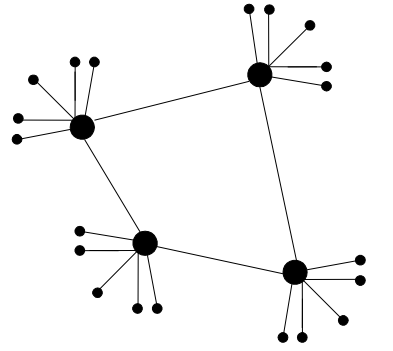
\includegraphics[width=0.5\textwidth]{immagini/Copertura_gerarchica.png}
              \caption*{Copertura gerarchica}
          \end{figure}
    \item Ogni file associato con un suo hash e un suo descrittore
    \item Client invia una query di keyword a suo group leader
    \item Group leader risponde con dei ``match'' del tipo
          \begin{center}
              $<$\emph{hash del file, indirizzo IP}$>$
          \end{center}
    \item Se leader inoltra la query ad altri leader, questi rispondono con altri match
    \item Il cliente sceglie quindi i file da scaricare
\end{itemize}

\paragraph{\emph{Reti strutturate}}

In una rete strutturata i nodi vengono organizzati seguendo un ben preciso insieme di regole, in modo da migliorare l'efficienza di alcune operazioni come, ad esempio, la ricerca di un particolare contenuto.\
L'aggiunta o la rimozione di nodi è un'operazione costosa.\
Un famoso protocollo che utilizza tecniche di questo tipo è BitTorrent.

\paragraph{Reti strutturate - DHT}

\begin{itemize}
    \item Sistemi con Distributed Hash Table (DHT)
    \item Ad ogni peer è assegnato un ID ed ogni peer conosce un certo numero di peer
    \item Ad ogni risorsa condivisa (pubblicata) viene assegnato un ID, basato su una funzione hash applicata al contenuto della risorsa ed al suo nome
    \item Routing della risorsa pubblicata verso il peer che ha l’ID più simile a quello della risorsa
    \item La richiesta per la risorsa specifica sarà instradata verso il peer che ha l’ID più simile a quello della risorsa
\end{itemize}

\subsection{BitTorrent:\ una rete P2P molto diffusa}

BitTorrent è un protocollo P2P progettato da Bram Cohen per la condivisione di file particolarmente voluminosi.\
Il termine \emph{condivisione} (sharing) in questo contesto è tuttavia usato in modo differente dai classici protocolli di condivisione di file.\
Non si ha semplicemente un peer che consente a un altro peer di prelevare un intero file:\ in questo caso è un gruppo di peer che collabora per fornire ad altri peer del gruppo una copia del file.\
La condivisione dei file avviene tramite un processo collaborativo chiamato \emph{torrent}.\
Ogni peer che partecipa a un torrent preleva parti del file (da 256 KB), chiamate chunk, da un altro peer e contemporaneamente trasmette i propri chunk ad altri peer che non li possiedono ancora.\
Questa divisione dei file permette di

\begin{itemize}
    \item ridurre il carico di ogni sorgente;
    \item ridurre la dipendenza dal distributore originale;
    \item fornire ridondanza.
\end{itemize}

\noindent Viene implementata una strategia chiamata \emph{tit-for-tat} (occhio per occhio) che assomiglia molto a quella di un gioco per bambini.\
L'insieme dei peer che fanno parte di un torrent viene chiamato \emph{swarn} (sciame).\
In uno sciame, un peer che possiede una copia dell'intero file viene chiamato \emph{seed} (seme); un nodo che ha solo una parte del file e desidera ottenere il file completo si chiama invece \emph{leech} (sanguisuga).\
Uno sciame è quindi composto da vari seed e leech.

\subsubsection{\emph{BitTorrent con tracker}}

BitTorrent nella versione originale prevede un ulteriore elemento detto \emph{tracker}.\
Questo, come indicato dal nome, tiene traccia delle operazioni dello sciame, come si vedrà in seguito.\
La Figura \ref{fig:BitTorrent} illustra un esempio di torrent con seed, leech e tracker.

\begin{figure}[H]
    \centering
    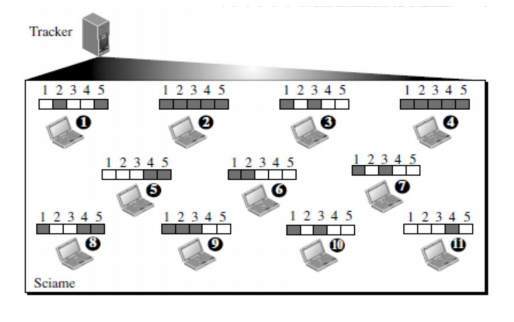
\includegraphics[width=0.7\textwidth]{immagini/BitTorrent.png}
    \caption{Esempio di torrent }
    \label{fig:BitTorrent}
\end{figure}

Nella figura il file da condivere è suddiviso in cinque chunk.\
I peer 2 e 4 possiedono già il file completo, gli altri ne hanno solo alcune parti:\ le parti possedute da un nodo nella figura sono ombreggiate.\
L'uploading e il downloading delle parti continua, mentre alcuni peer possono abbandonare il torrent e altri peer possono aggiungersi.

Si supponga ora che un nuovo peer voglia scaricare proprio quel file:\ contatta un motore di ricerca specializzato indicando il nome del file e riceve un metafile, chiamato \emph{file torrent}, che contiene le informazioni relative alla suddivisione in parti del file e l'indirizzo del tracker che gestisce quel particolare torrent.\
Il nuovo peer può ora contattare il tracker per ricevere l'indirizzo di alcuni peer nel torrent, solitamente chiamati \emph{vicini} (neighbor).\
Il nuovo peer è ora parte del torrent e può iniziare a scambiare chunk.\
Ottenuto il file completo di tutte le sue parti, può abbandonare il torrent oppure contribuire ad aiutare gli altri peer, inclusi quelli che si sono uniti al torrent dopo di lui, ad ottenere tutte le parti del file.\
Un peer può anche abbadondare il torrent prima di avere ottenuto tutte le parti del file, per riagganciarsi eventualmente in un momento successivo.

Sebbene i meccanismi di accesso, condivisione e abbandono di un torrent possano sembrare molto semplici, il protocollo BitTorrent utilizza un insieme di politiche per garantire equità, per incoraggiare i peer a partecipare attivamente allo scambio, per evitare di sovraccaricare un peer con troppo richieste e per consentire ai peer di effettuare scambi alla velocità più ampia possibile.

Per evitare di sovraccaricare un peer e garantire un certo livello di equità, ciascun peer generalmente non può avere più di quattro vicini con cui effettuare scambi.\
I peer inoltre classificano i vicini come \emph{choked} (soffocati) oppure no, e come \emph{interested} (interessati allo scambio) oppure no.

Ogni peer divide i propri vicini nei quattro gruppi derivanti dalle combinazioni di:\ choked oppure no, interested oppure no.\
Il gruppo non choked è quello al quale il peer attualmente è connesso e con il quale scambia chunk.\
Il gruppo chocked invece è l'insieme dei vicini ai quali non è attualmente connesso ma potrebbe connettersi in futuro.

Ogni 10 secondi ogni peer controlla uno dei peer nel gruppo degli interessati ma soffocati per verificare se può ottenere una migliore velocità di trasferimento.\
Se questo peer ha una velocità superiore a uno qualsiasi dei peer non soffocati entra a far parte di quest'ultimo gruppo, mentre il peer non choked con la velocità più bassa viene spostato nel gruppo dei soffocati.\
Così facendo i nodi nel gruppo non soffocato sono sempre quelli con la migliore velocità tra quelli controllati.\
Questa strategia divide i vicini in sottogruppi, nei quali i nodi vicini con velocità di trasferimento dati compatibile comunicano l'uno con l'altro.\
In questo meccanismo si può vedere l'implementazione della strategia di scambio tit-for-tat menzionata in precedenza.

Per consentire a un peer, che è appena entrato in uno sciame ma che non ha ancora nulla da condividere, di ricevere chunk dagli altri partecipanti, viene implementata una politica di \emph{unchoking ottimistico}.\
Significa che tutti i peer promuovono casualmente, ogni 30 secondi, un peer dal gruppo soffocato, indipendentemente dalla sua velocità di uploading, inserendolo nel gruppo dei non soffocati.

Inoltre, il protocollo di BitTorrent cerca di bilanciare il numero di chunk che ogni peer possiede in ciascun istante utilizzando una strategia chiamata \emph{rarest-first} (prima il più raro).\
Questa strategia prevede che ogni peer tenti per prima cosa di prelevare le parti con il minor numero di copie esistenti fra i vicini.\
Così facendo, i chunk rari vengono scambiati molto rapidamente e si giunge in fretta a una distribuzione piuttosto omogenea.
